\documentclass[11 pt]{article}

\usepackage{titlesec}
\usepackage[dvipdfmx]{graphicx}
\usepackage{bmpsize}
\usepackage{amsmath,mathrsfs}
\usepackage{amssymb}
\usepackage{enumerate}
\usepackage{grffile}
\usepackage{hyperref}
\usepackage{dsfont}
\usepackage{url}
\usepackage{ifplatform}
\ifwindows
	\usepackage{graphicx}
	\usepackage{epstopdf}
\fi
\hypersetup{
    colorlinks,
    citecolor = black,
    filecolor = black,
    linkcolor = black,
    urlcolor = black
}
\usepackage[margin=1in]{geometry}
\usepackage[font={scriptsize}]{caption}
\usepackage{listings}
\lstset{
basicstyle=\small\ttfamily,
columns=flexible,
breaklines=true
}

\title{Lab Notes for Compressed Sensing Coding}

\makeatletter
\renewcommand\paragraph{\@startsection{paragraph}{4}{\z@}%
            {-2.5ex\@plus -1ex \@minus -.25ex}%
            {1.25ex \@plus .25ex}%
            {\normalfont\normalsize\bfseries}}
\renewcommand\subparagraph{\@startsection{subparagraph}{5}{\z@}%
            {-2.5ex\@plus -1ex \@minus -.25ex}%
            {1.25ex \@plus .25ex}%
            {\normalfont\normalsize\bfseries}}
\makeatother
\setcounter{secnumdepth}{5} % how many sectioning levels to assign numbers to
\setcounter{tocdepth}{5}    % how many sectioning levels to show in ToC
\setcounter{section}{-1}

\newcommand{\me}{\mathrm{e}}
\newcommand*\diff{\mathop{}\!\mathrm{d}}
\newcommand{\ep}{\varepsilon}
\newcommand{\sectionbreak}{\clearpage\newpage}
\newcommand{\mitem}{\item[--]}
\newcommand{\bo}{\noindent\textbf}
\newcommand{\etal}{\emph{et. al.}}
\newcommand{\matlab}{\textsc{Matlab }}
\let\oldsection\section
\renewcommand\section{\clearpage\newpage\oldsection}

\usepackage[nodisplayskipstretch]{setspace}
\usepackage{fancyhdr}
\pagestyle{fancy}

\fancyhead[R]{Salerno}
\fancyhead[C]{Lab Notes for Compressed Sensing Coding}
\fancyhead[L]{MICe}

\begin{document}

\vfill

  \begin{titlepage}
    \vspace*{\fill}
    \begin{center}
      {\huge {Lab Notes for Compressed Sensing Coding}}\\[0.5cm]
      {\large {Anthony Salerno}}\\[0.4cm]
      February 17, 2015 - \today
    \end{center}
    \vspace*{\fill}
  \end{titlepage}

\clearpage
\newpage

\tableofcontents

\newpage

% Section 0
\section{Questions for Brian}
  Here, I will include questions that I asked Brian based on the date of the meeting -- I'll also include a basic description of the topic within the subtopics for each set of questions and whatnot.

  \subsection{Direction Based Gradient in the Objective Function}
    \begin{enumerate}
      \item The values that we get here are somewhat dependent on how many different directions we take. It's noted that this can be changed on the fly (which is nice) but what should be our default ``threshold" of the dot product to accept?

      \item The values coming from this set are on the order of $10^{14}$, meanwhile, the gObj is an order of magnitude lower, and the TV and XFM are on the order of $10^9$. Do we need to normalize this value by the number of directions that we get?

      \item For some reason, even though as a sum, the values should only be on the order of $10^{14}$, the summation of all of these terms gives a value on the order of $10^{16}$. This needs to be looked into. Regardless, this value is HIGH in comparison to our data ($10^4$), should this be of concern?

      \item How should we change our analysis methods so that the XFM and TV weightings are comparable to the objective, and thus will actually have an effect?

      \item What should we do to make the objective difference less. In the Shepp-Logan, the values are significantly lower (unless this is merely a by-product of having voxel values of $\sim10^4$)
      \end{enumerate}


% Section I
\section{Proof of Principle (02.17.15 - 02.23.15)}

  \subsection{Introduction}
    Beginning work on the ``Proof of Principle" as per the 12.19.14 Meeting Notes - Plan 2

    The notes state that we are to:
    \begin{itemize}
      \item Pick one slice - extract slice from dataset with FT on RO (i.e. in dim space) and no FT on PE1 and PE2 (aka PE and SL)
      \item Isotropic undersampling (I think this is a bad idea)
      \item Recon slices independently with Lustig code (using $\lambda_2 Psi[m] + \lambda_1 TV[m]$)
      \item Add a directional similarity term to the recon (so we can recon similar slices simultaneously) ($\lambda_3 ||m_j - m_k||_2 f(\vec{d_j} \cdot \vec{d_k}))$
      \item However, the form of $f((\vec{d_j}\cdot \vec{d_k}))$ is still unknown
      \end{itemize}

    \noindent Note that the git repository for this work can be found at \url{https://github.com/aasalerno/Lustig}. For pre-emptive notes on the code that Lustig wrote, please see \verb!demo_SheppLoganTV_Notes.txt!. \\ \\

  \subsection{Preamble...}
    
    \subsubsection{Hypothesis}

        To begin, today we should be able to get a decent code running that can do Lustig's code on any specified slice that we choose. I expect that the code will work as expected and provide a good rendition of the undersampled data with minimal alterations required. The hope is that we can use the basis of the code as an engine (that will need some optimization) in order to work with the data as we so hope.

    \subsubsection{Notes - Unpolished}
        First spent a ridiculous amount of time getting \LaTeX up and running on this computer... But it works now! 

        The code is written both on my computer as well as on the lab computers -- via a central git on git-hub -- using the same datasets as required. The datasets in use are Jacob's data, reconstructed purely using the standard recon algorithm (that is, no \matlab involved).

        For all pushes and pulls, see the git-hub repository. There are many (and it can be mapped by day!)

        The code is to be written such that it is built and any values that are above 1-sampFac will be included. This means that when we are actually tacking on the $r$ correction, we need to do it as $1-\frac{r}{\text{max}(r)}$

        Seem to have a problem with the values that I'm getting. The outer portions of k-space seem to have almost no chance of being chosen. With a penalty threshold of only 0.25 (given a sampFac of 0.5), only 40\% of values are chosen. Most of the lost points are on the corners of $k$-space, so this may be ok... However, I need to look into \textbf{possibly making the CS type sequence specific, for things like cylindrical acquisition}. \\ \\ 
      
        \noindent Date: 02/20/15 \\
        As of about 11:00 (commit 6a9cfb111c508df0af9a7222ba277ef118ba147), the code \verb!testMap.m! is up and running. It will be used in order to actually build the map of what we are undersampling and then this will be pumped into an adapted version of Lustig's code in order to get it up and running.

        Encountered a bit of an issue with how the data is obtained. Since this information is only the magnitude of the data, I'm going to make a version that can handle taking the real and imaginary parts of the data, then feeding that through to the next set of functions.

        As of 12:08 PM, functionality has been added for the function to handle two files containing the real and imaginary parts of the $k$-space information!

        Now, we want to add in the CS part of the code. Here is where things become a little painful, but we can look at the datasets and actually do what is done in CS.

        For some unapparent reason, the code doesn't seem to want to work. This is really annoying and irritating as the error seems to be stemming from the raw files, which may render a tonne of previous work that I've done utterly useless. Ok, scratch that -- the issue was my method of plotting. I wasn't plotting the abs of the data. 

        As of about 5:00 it is working. I'm going to git push it and go home. \\ \\

        \noindent Date: 02/23/15

       Upon a first look at the code that I wrote last week (adapted from \verb!demo_SheppLoganTV.m!, the code doesn't seem to have too great of an effect. The differences between the ``im\_dc" (density corrected original) and the CS reconstructed data is on the order of $10^{-9}$, when the data is on the order of 1.

        \begin{itemize}
          \item One of the first things that I should try is to change the TV and L1 penalties as they are currently set to 0.01 each. This may be too low to have an effect on real data -- the code that I am adapting from is using a numerical phantom.
          \item The next step would be to try different slices or different data. Perhaps the noisiness of this data is causing a problem, but can be fixed with some more phase corrections.
        \end{itemize}

        I changed the values of the two penalties ($\lambda_1$ and $\lambda_2$), increasing them by a factor of 10, each becoming 0.1. The overall residual became a little bit larger, but is still on the order of $10^{-9}$, which is negligible.

        In order to make the data make a bit more sense (i.e. make sure I'm not making a stupid mistake on how I'm building the filter, etc.) I'm going to use Lustig's method of building the undersampling pattern.

        I changed the code \verb!testMap.m! pretty substantially, so see git-hub for a previous version. The alterations were made to try and use the other undersampling pattern. One thing that I may do later is alter Lustig's PDF that is produced by tacking on the directionality afterwards.

        After changing to Lustig's method of undersampling, we see some bigger differences, but, the undersampling kind of makes it look pretty bad. It may be how the FT (using this `\verb!p2DFT!') instead of just doing an FFT as it is done in \matlab. This seems like something weird that they don't need to do, as it just makes the data look bad... Though there must be a reason for this

        As it stands -- 4:00PM 02/23/15 -- this is as far as I can go without further understanding how well everything is going to work for the perpendicular and parallel to the gradient direction for the undersampling technique.

    \subsection{Simulations}

      \subsubsection{Preamble}

        Here what we want to ensure is that by applying specific filters, we are obtaining what we expect. The expectation is that using a mask that is parallel to the gradient direction (applied in $k$-space) is going to look significantly worse than a mask applied perpendicular to the gradient direction.

    \subsection{Hypothesis}
      Using a simulation, we will be able to tell distinct differences between the use of the two different maps. The map using a perpendicular mask on the undersampled $k$-space will look better than the data undersampled using the parallel mask, as the smearing will not be as bad in the cross direction of the diffusion.

      The code is written in \verb!buildLambda.m!. It is currently built just to handle a 2D case and then \emph{eventually} handled to build a 3D. In order to make it work with the code, an idea is to make it have a $z$-stack (in our case, a $y$ stack, or a `read-out" stack). \\ \\ 



% Section II
\section{Analysis of CS Code -- Sanity Check (03.10.15)}
  \noindent Date: 03/10/15

  \subsection{Preamble...}

    As of this point, I've finally given my seminar (which apparently went well!) and now, I'm trying to see if there's something inherently wrong with how I'm running my CS codes, as they aren't producing the effects that I would expect. The noise looks \emph{really} weird, and isn't how I'd expect it to be.

    So, for today, we are going to change things up a bit, and move on to try and understand exactly what's happening in this code -- I will try to include figures where I believe it makes sense due to the simplicity of doing so.

    In order to simplify things, I made a file using the raw data from Jacob's Diffusion Weighted Imaging data taken on July 29, 2014. The raw data files are located in \\ \verb!/projects/muisjes/asalerno/CS/data!. Specifically we are using brain 10, direction 32. This brain was chosen to be the simplest of cases, as this is a $b_0$ scan, thus there is no expected major differences because of the lack of diffusion weighting.

  \subsection{Down-sampling}

    One \emph{major} thing to note is the effect that down-sampling has. We can see it here:

    % Effects of downsampling figure
    \begin{figure}[h] 

      \centering
      \vspace{0pt}
      \setlength\fboxsep{0pt}
      \setlength\fboxrule{0.5pt}
      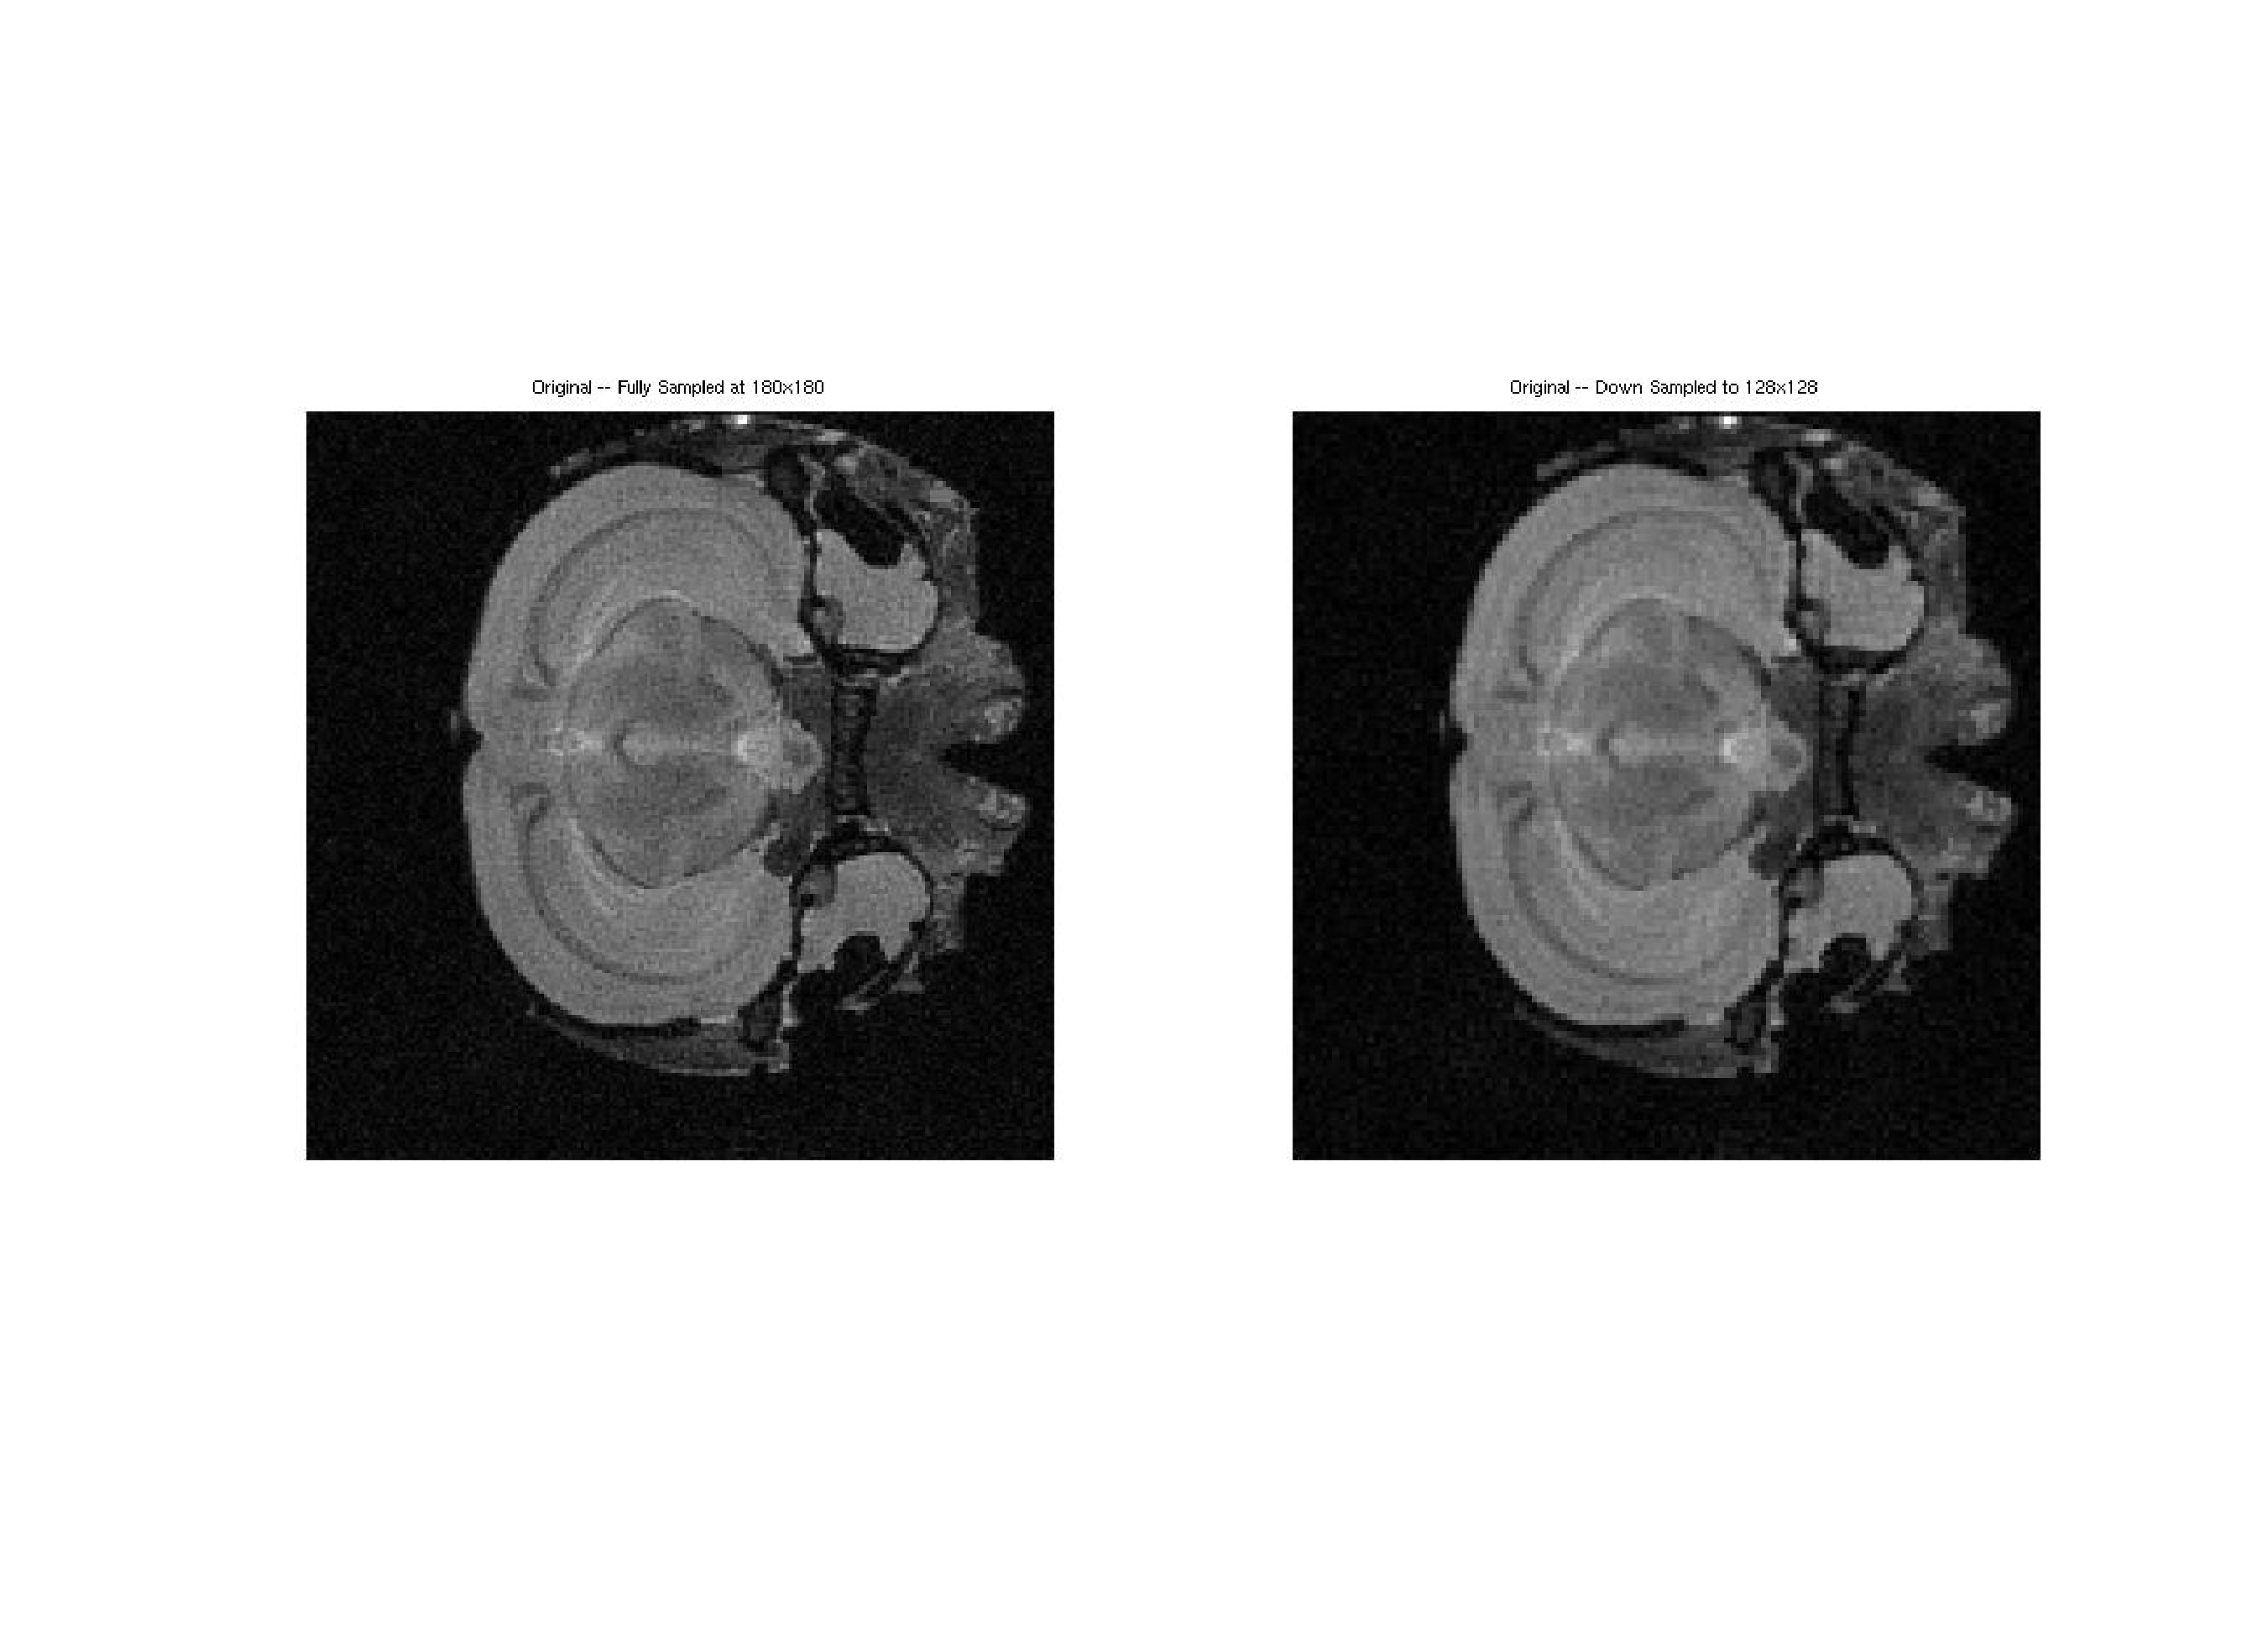
\includegraphics[trim = {60mm 100mm 46mm 70mm},clip,scale = 0.4] {Figs/CS_DTI_Sims/FullvsDownSample.eps}
      \caption{We can see the significant blurring effect that downsampling the figure to be 128x128 has. The blurring cannot be fixed, as in order to do this, we must sacrifice some higher spatial frequency information. Note that this is using \matlab blurring. This is explained further in the next section and figure 2.}
      \label{fig:dwnsamp}

      \end{figure}

    The downsampling is absolutely required because of how the wavelet transform is done. The 2D Wavelet transform has a $2^n$ size requirement in order to work (Lustig 2007, Yang 2015). We don't particularly care about the number of slices being $2^n$ as this will be fully sampled anyway. 

    It seems like \matlab does something a little weird with how it downsamples the FFT... It produces what looks like just a blurred copy of the image (as seen above) but it doesn't seem to get the data from the centre, but instbuildLambdaead chooses the data in the top right section (before shifting) preferentially. This can be seen in Figure 2.

    \newpage
    \begin{figure}[h] 

      \centering
      \vspace{0pt}
      \setlength\fboxsep{0pt}
      \setlength\fboxrule{0.5pt}
      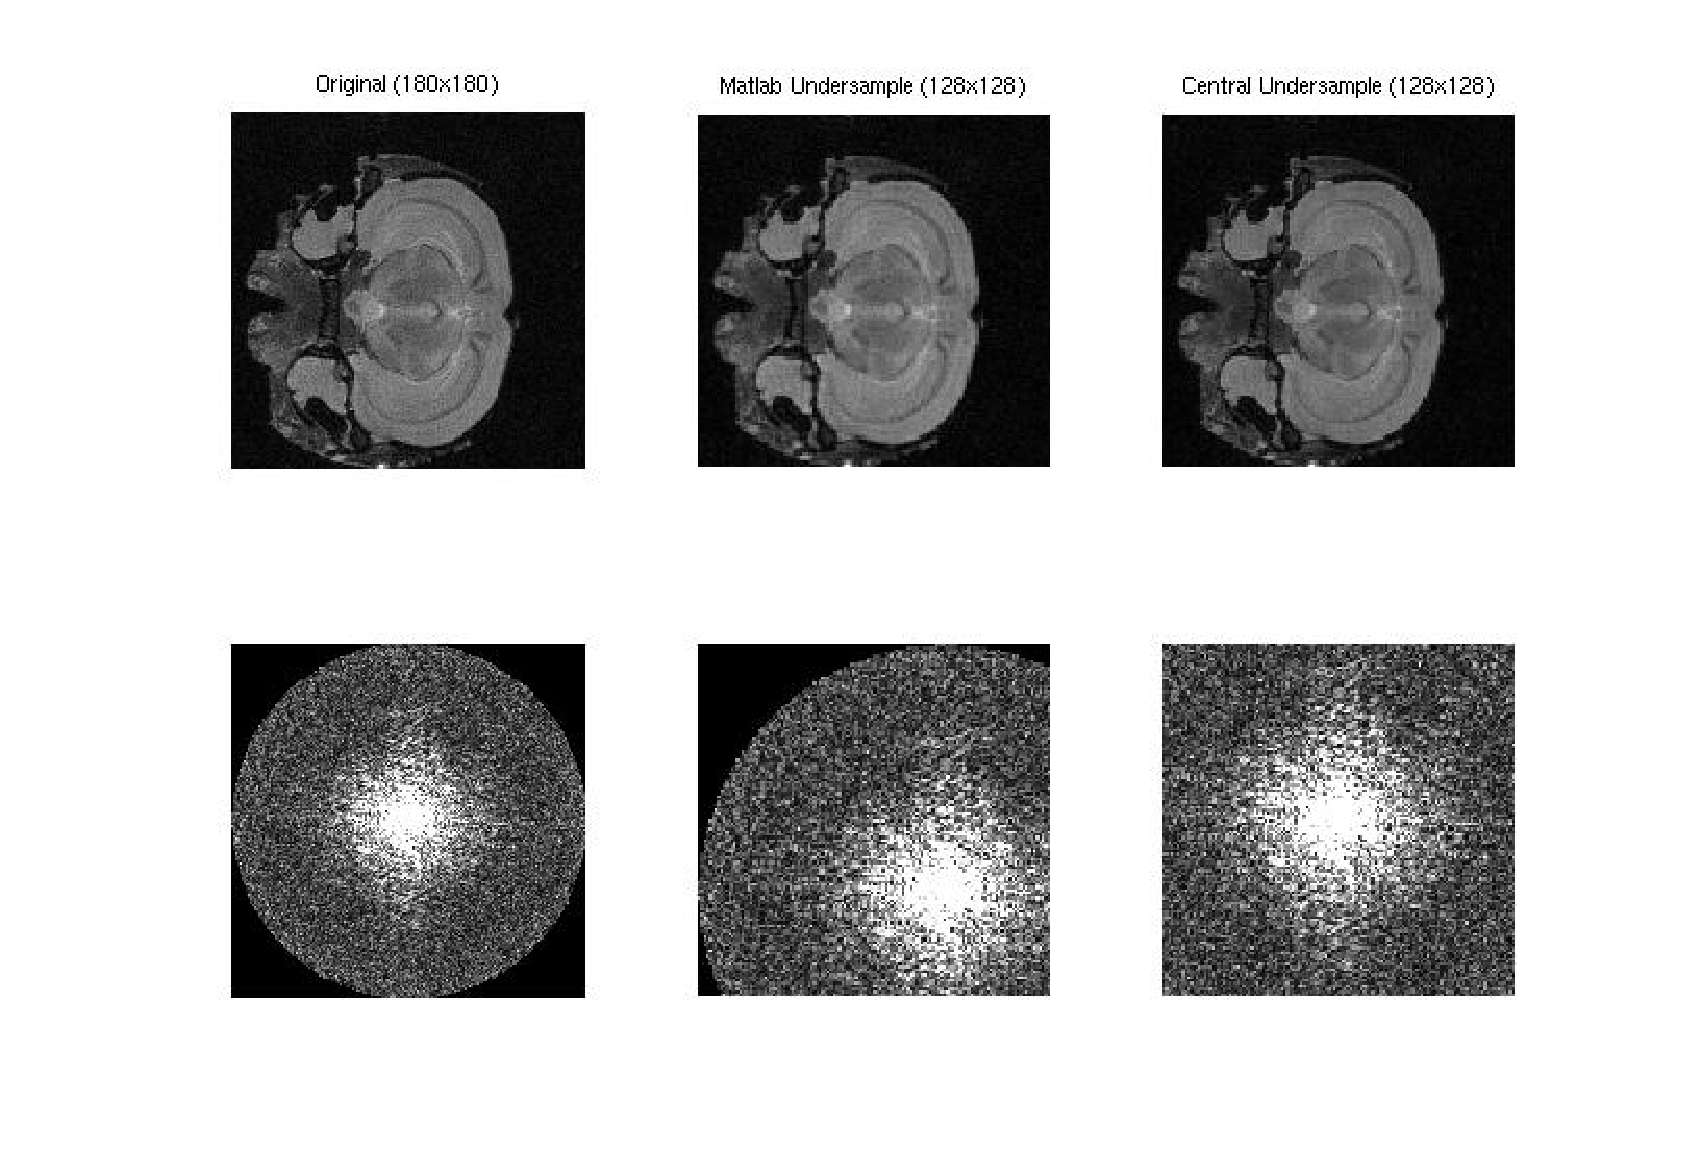
\includegraphics[trim = {36mm 20mm 20mm 8mm},clip,scale = 0.6] {Figs/CS_DTI_Sims/FullvsMatvsCent.eps}
      \caption{In this figure, we see some small differences between the method of undersampling done in \matlab vs a logical undersampling method that takes the data from the centre of $k$-space. All data here taken from slice 150 \emph{after} doing a 1D FFT in the readout direction.}
      \label{fig:matvscent}

      \end{figure}

    We can see in the above figure that \matlab does something really weird and so, we will be using my method in order to do reconstructions that alter the number of voxels per dimension.

    In order to make sure that we're using the right one, the file we must use is \verb!kspaceDS.10.32.mat!, as this is the dataset that has been undersampled properly. For this work, what we will do right now, is look at how we can try to do a reconstruction properly using compressed sensing. We may be able to do this logically using some of the existing work here. In the angiography case, they use the previous slice as the base image as ``not much is expected to change". We can do better than this, as we can try to do a combined reconstruction, where the $b_0$ average of the same slice (to start) would be the same. 



% Section III
\section{Simulations - (03.11.15 - 04.01.15)}
  \noindent 03.23.15 (work completed on and before 03.19.15)
  
  \subsection{Preamble}

    The point of running this simulation is to see what the best undersampling method to use would be. Our plan of attack is to do this experiment two fold, firstly with purely numerical data -- i.e. a ``phantom" that I design, and then afterwards using true brain data and seeing if we can get an understanding of what the best method would be. 
    
    Some of this information is noted at an earlier point in time, 

  \subsection{Hypothesis}

    The expectation is that the best style would be to use the ``parallel to the gradient direction" as this will give us the sharpest edge information in order to tell a cross section of the fibres that we are expecting to see. The worst should be the ``perpendicular" case. It is noted that our nomenclature from before was misleading. In order to ensure that we have it correctly, the following figure explains what is meant by each.

    % Directionality! figure
    \begin{figure}[h] 

      \centering
      \vspace{0pt}
      \setlength\fboxsep{0pt}
      \setlength\fboxrule{0.5pt}
      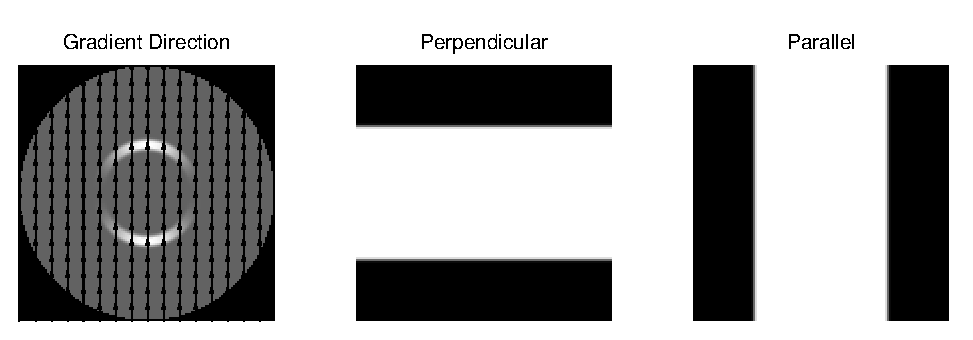
\includegraphics[trim = {0mm 0mm 0mm 0mm},clip,scale = 0.8] {Figs/numericalSims/GradDir01.eps}
      \caption{We can see the direction of the gradient in the left-most panel, and the definitions of the others. The parallel will give us the ``cross-fibre" information mostly, and the perpendicular will give us the ``along the fibre" information.}
      \label{fig:GradDir}

      \end{figure}

  \subsection{Results}
  
    \subsubsection{Numerical Simulations}
    
      For the numerical simulations, we started with a phantom that was comprised of three parts. The phantom can be seen in the following image.
    
      \begin{figure}[!h] 

        \centering
        \vspace{0pt}
        \setlength\fboxsep{0pt}
        \setlength\fboxrule{0.5pt}
        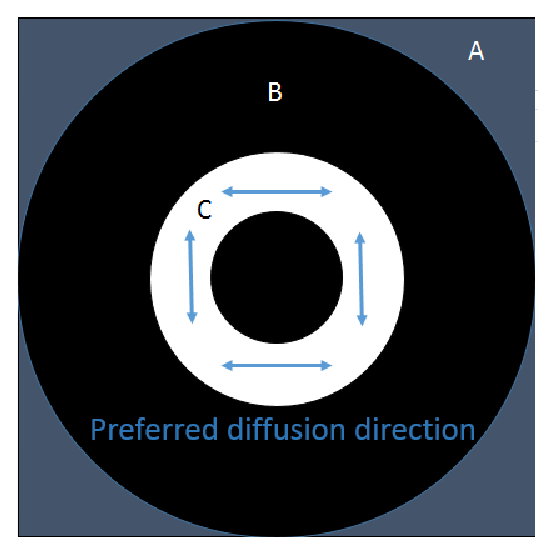
\includegraphics[trim = {0mm 0mm 0mm 0mm},clip,scale = 0.8] {Figs/numericalSims/Phantom.eps}
        \caption{This figure is the numerical phantom that we used. Region (A) represents an area of all zero data, used to serve as a reference point when plotting the figure (it forces the dynamic range to begin at zero). Region (B) represents an area of isotropic diffusion, where $\lambda_1 = \lambda_2 = \lambda_3 = 10^{-3}$. This area should have an FA value of zero. Region (C) represents an area with restricted diffusion, where $\lambda_1 = 10^{-3}$, but $\lambda_2 = \lambda_3 = 5 \times 10^{-4}$. This gives a theoretical FA value of approx $0.41$. It is noted that the $b$ value used in this experiment was 1917 $\frac{\text{s}}{\text{mm}^2}$}
        \label{fig:NumPhant}

        \end{figure}
    
    
      When we worked with this data, we used multiple different types of undersampling filters, and compared them to the fully sampled case. The ones that we used are:
      \begin{itemize}
        \item Circle
        \item Square
        \item Parallel Strip
        \item Perpendicular Strip
        \item Parallel Ellipse
        \item Perpendicular Ellipse
        \end{itemize}

      For the two ellipses, it is noted that the long axis to short axis ratio was set to be 2 (i.e. a/b = 2 if $\left(\frac{x}{a}\right)^2 + \left(\frac{y}{b}\right)^2 = 1$). It is also noted that $x$ and $y$ here are those of the axis rotated relative the gradient vector direction.
    
      % Talk about this more.
      Upon comparing all of our datasets, we found that the square and the circle gave the smallest RMS error. This can be seen via a bar chart -- this chart combined all the ROIs from all directions (doing the fully sampled - undersampled), and and ran an RMS on all of the data.
    
      \begin{figure}[!h]
        \centering
        \vspace{0pt}
        \setlength\fboxsep{0pt}
        \setlength\fboxrule{0.5pt}
        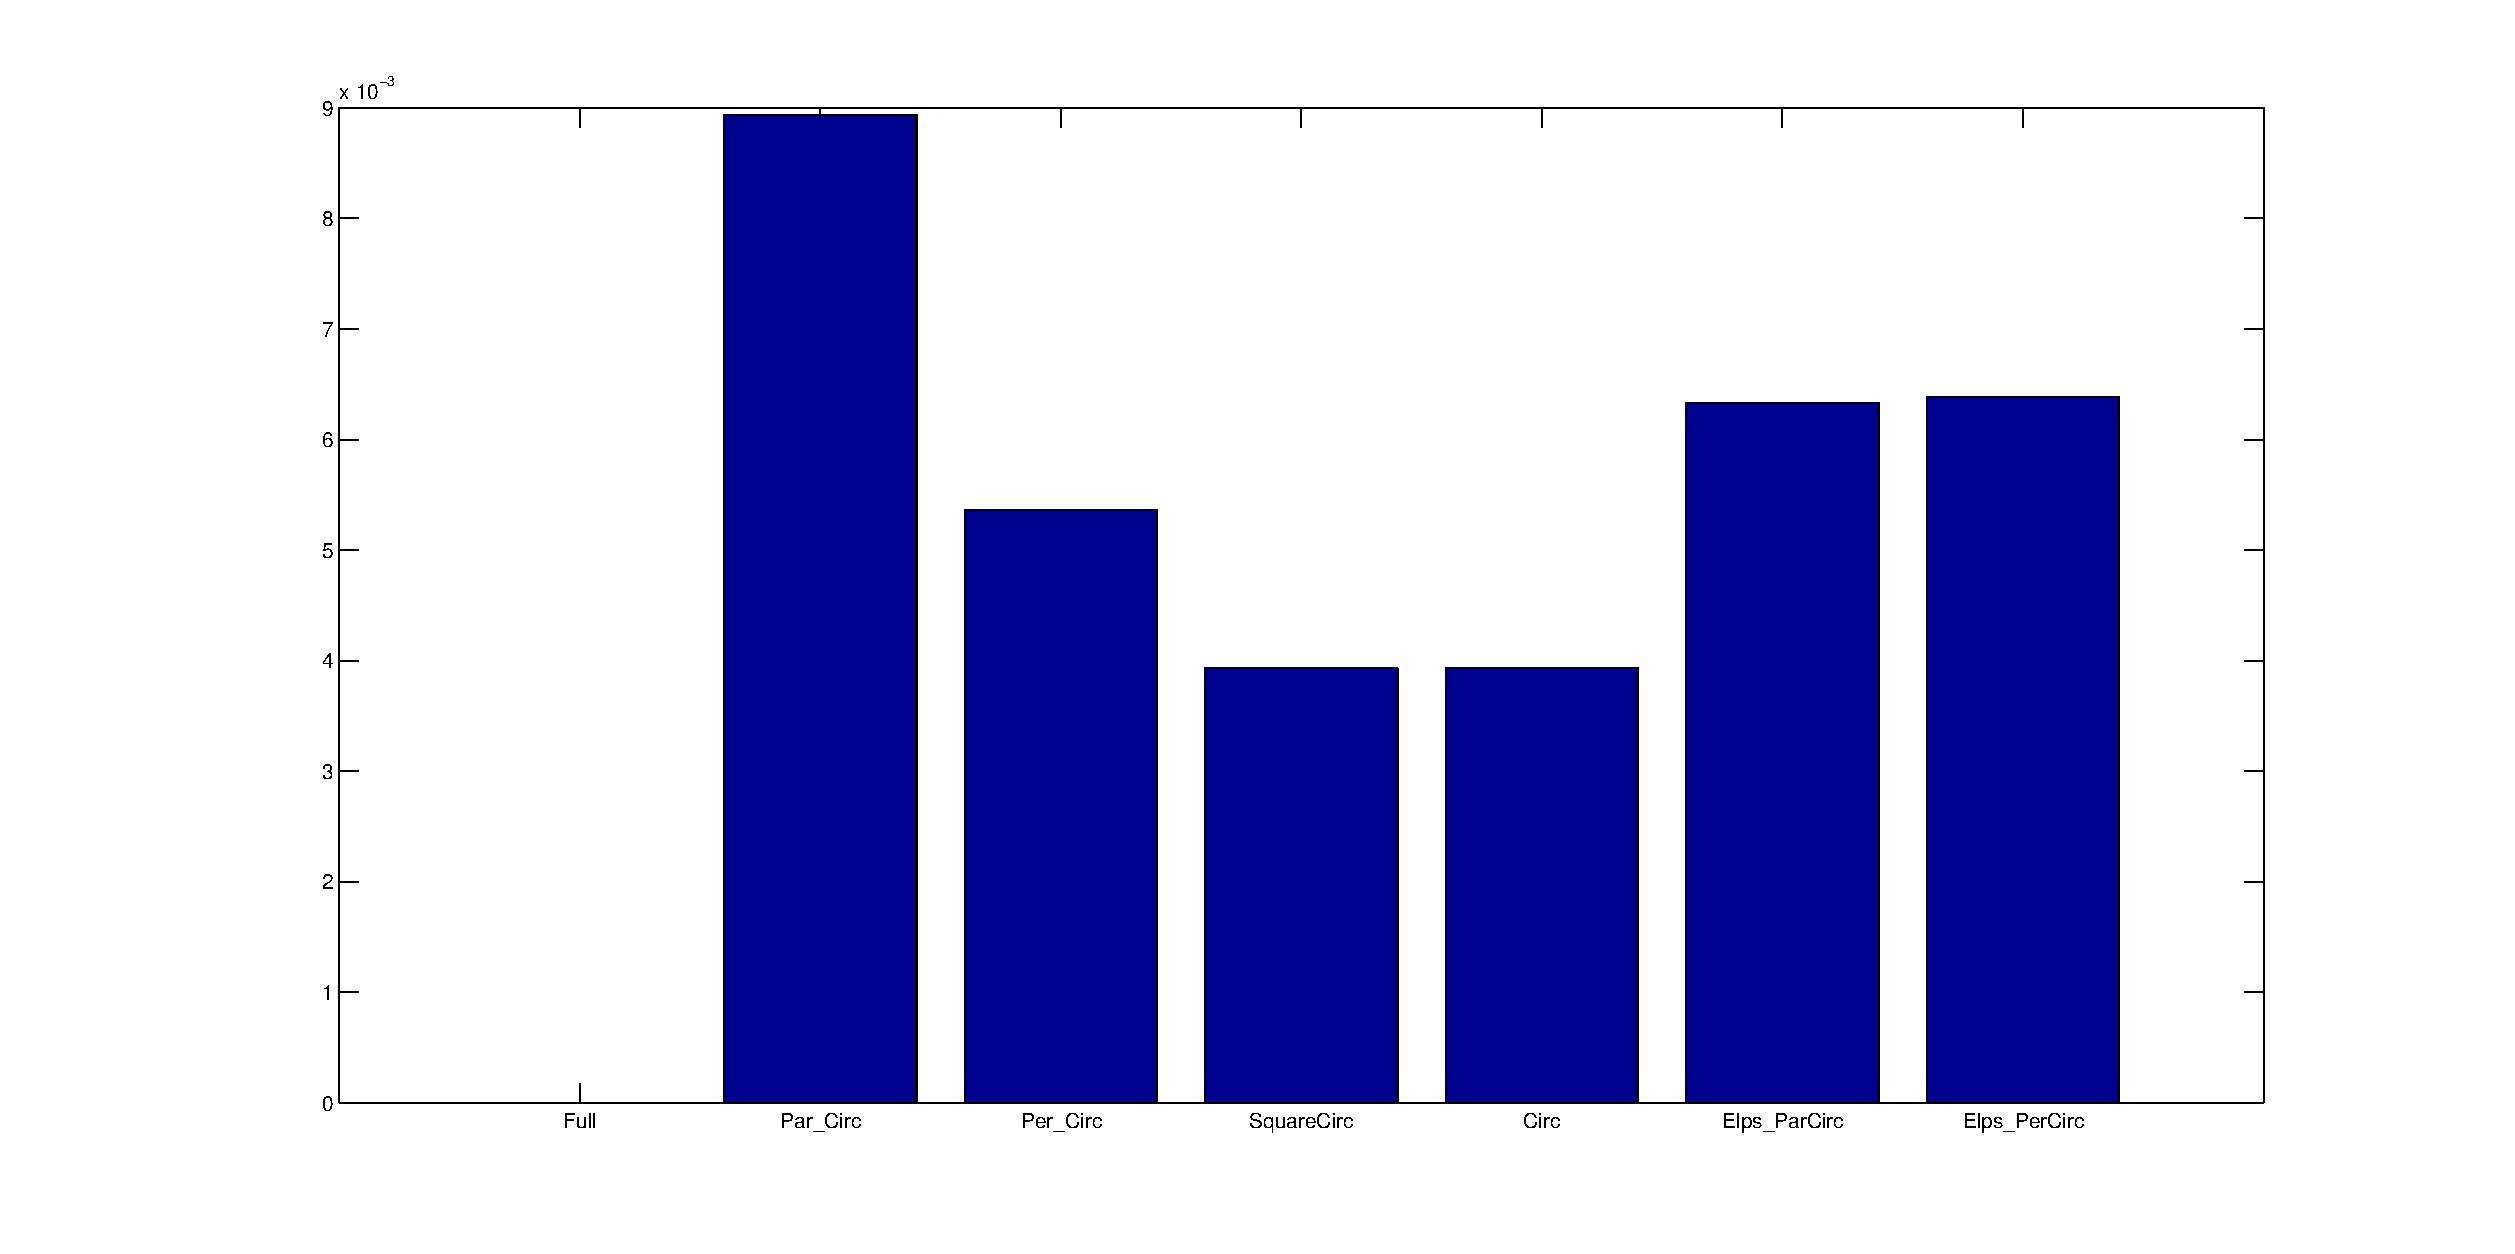
\includegraphics[trim = {10mm 0mm 10mm 0mm},clip,scale = 0.4] {Figs/numericalSims/nSimRMS.eps}
        \caption{This figure shows us how the RMS differs for the different undersampling types. We can see the undersampling types in the next figure.}
        \label{fig:RMSPhant}

        \end{figure}
    
      For these plots, we used a ROI that just covered the circle -- quite tightly -- so that we didn't have much of a confounding factor. We still saw, though, that the ``circle in the centre" (as seen in the next plot) was the best method to reduce the error that we get in our data.
    
      \begin{figure}[!h]
        \centering
        \vspace{0pt}
        \setlength\fboxsep{0pt}
        \setlength\fboxrule{0.5pt}
        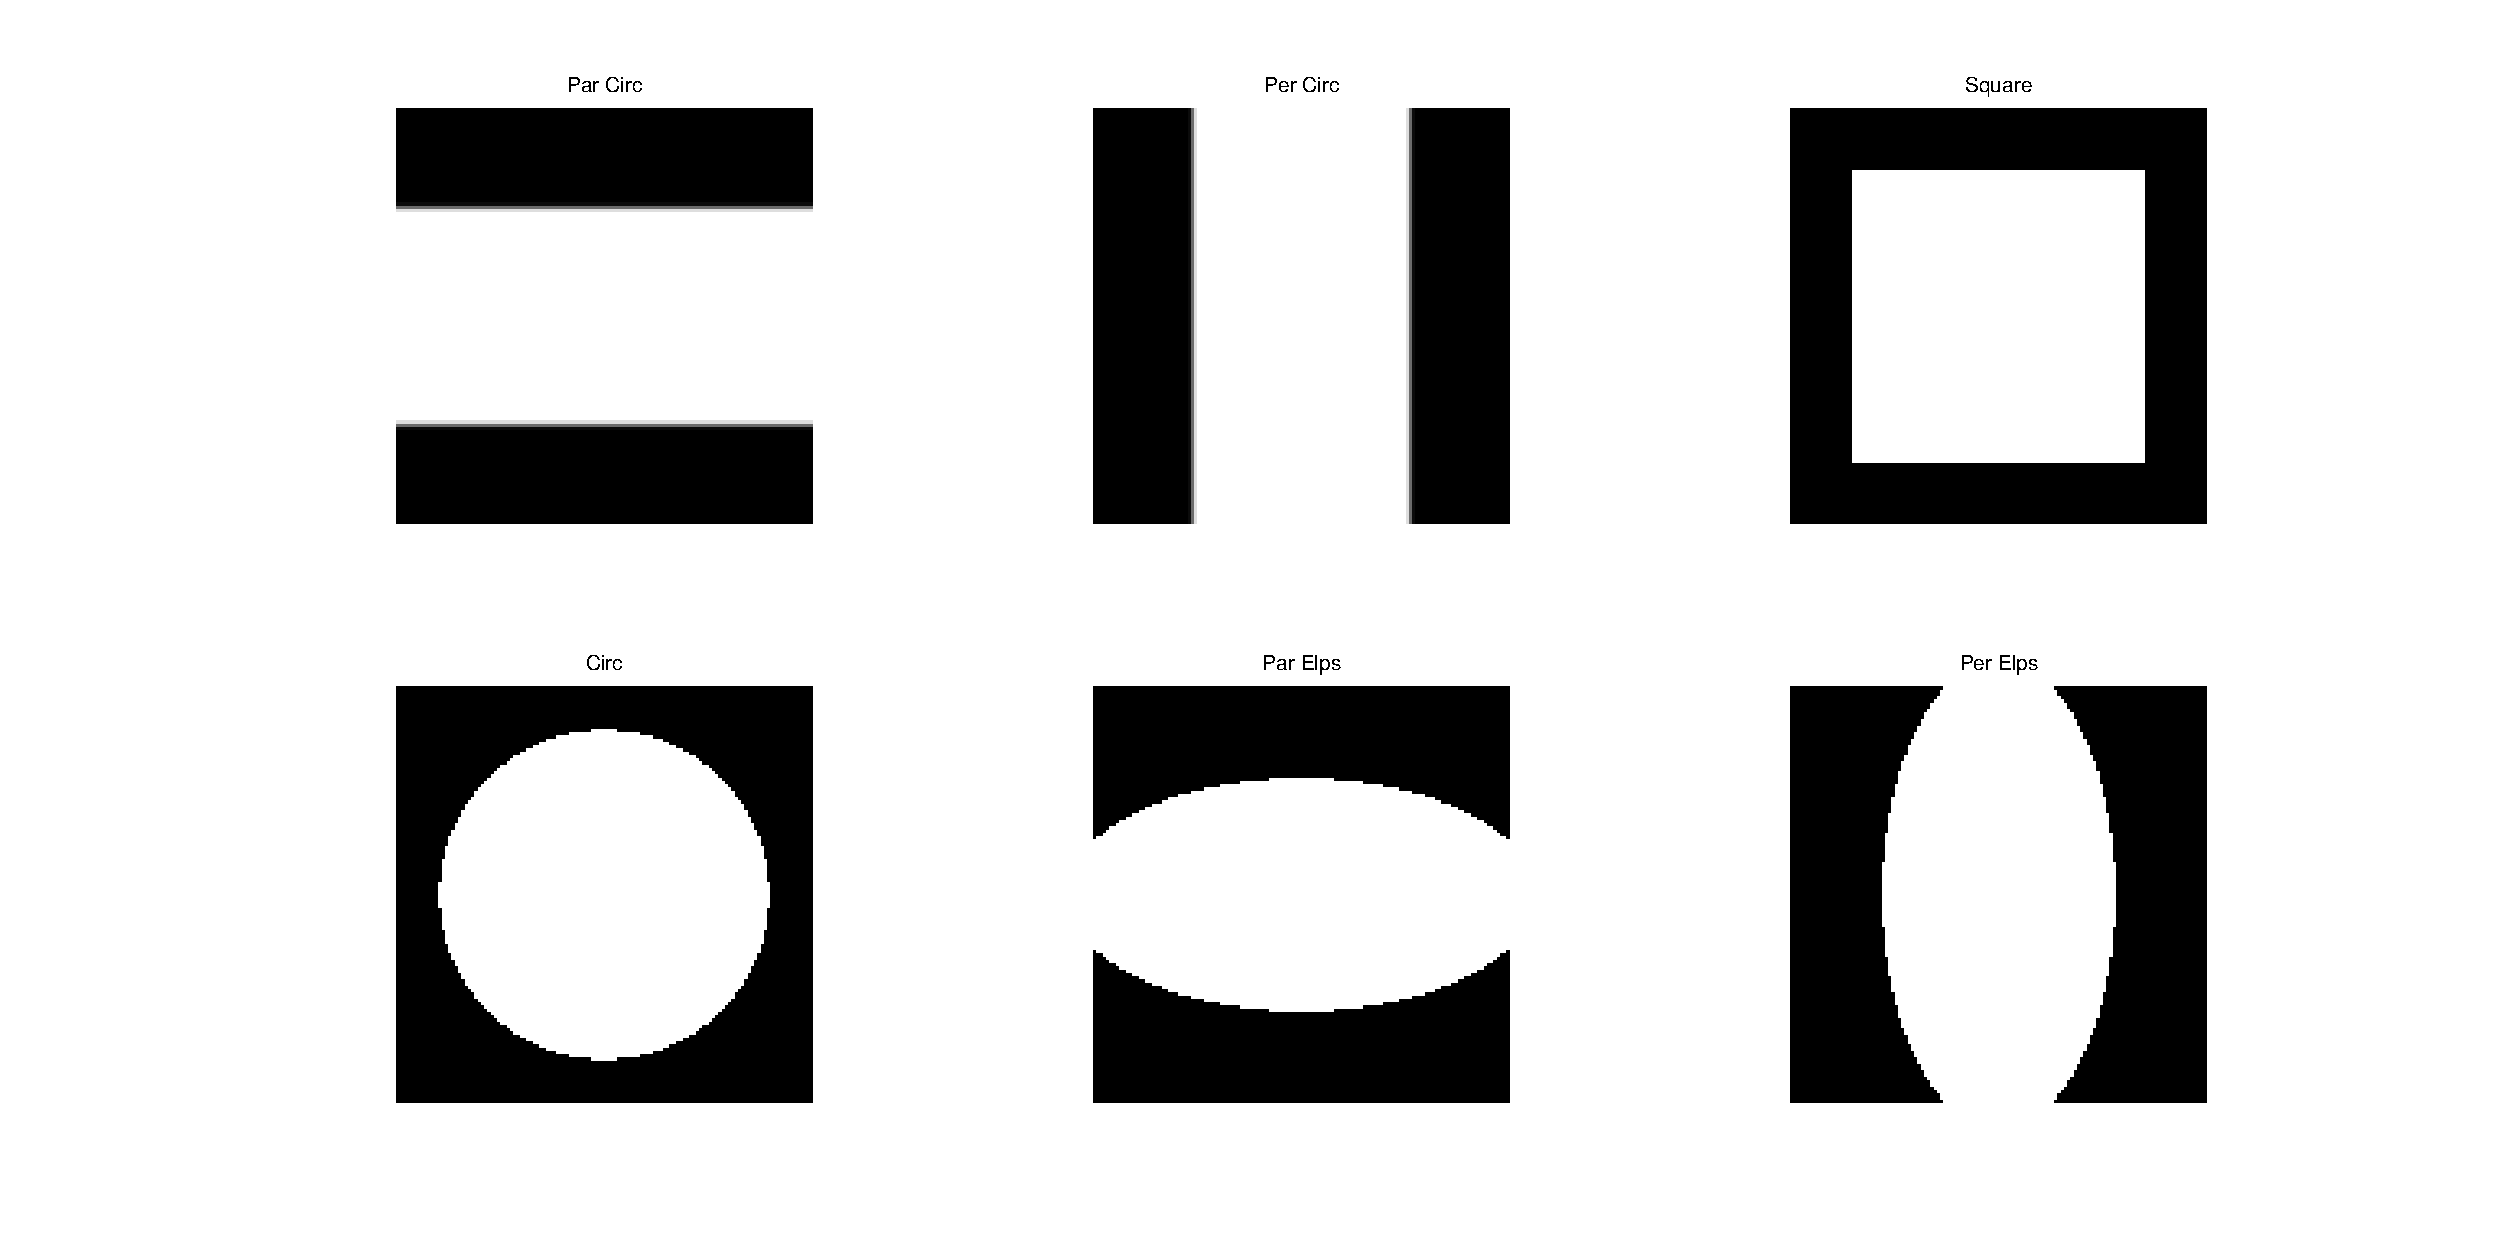
\includegraphics[trim = {10mm 0mm 10mm 0mm},clip,scale = 0.4] {Figs/numericalSims/DiffFilts.eps}
        \caption{The different filters that we used for the plots. It is noted that the codes used almost no roll off. For this example, we are assuming the gradient direction to be totally vertical.}
        \label{fig:USFilts}

        \end{figure}
    
      

      \newpage

    \subsubsection{Brain Data}
    
      When proceeding to brain data, I expect that we would be the same results. Using data that can be found in \verb!/projects/muisjes/asalerno/CS/data!, and undersampling methods that can be found in \verb!/micehome/asalerno/Documents/CompressedSensing!, we ran the same undersampling techniques, but got some interesting results. The ellipse method is now \emph{worse} than the strip method! Reasons for this are currently unknown. The dataset being shown is brain 2, all 30 directions, however, this can (and will) be redone for more brains in order to get a more realistic understanding of what's happening.
      
      \begin{figure}[h]
        \centering
        \vspace{0pt}
        \setlength\fboxsep{0pt}
        \setlength\fboxrule{0.5pt}
        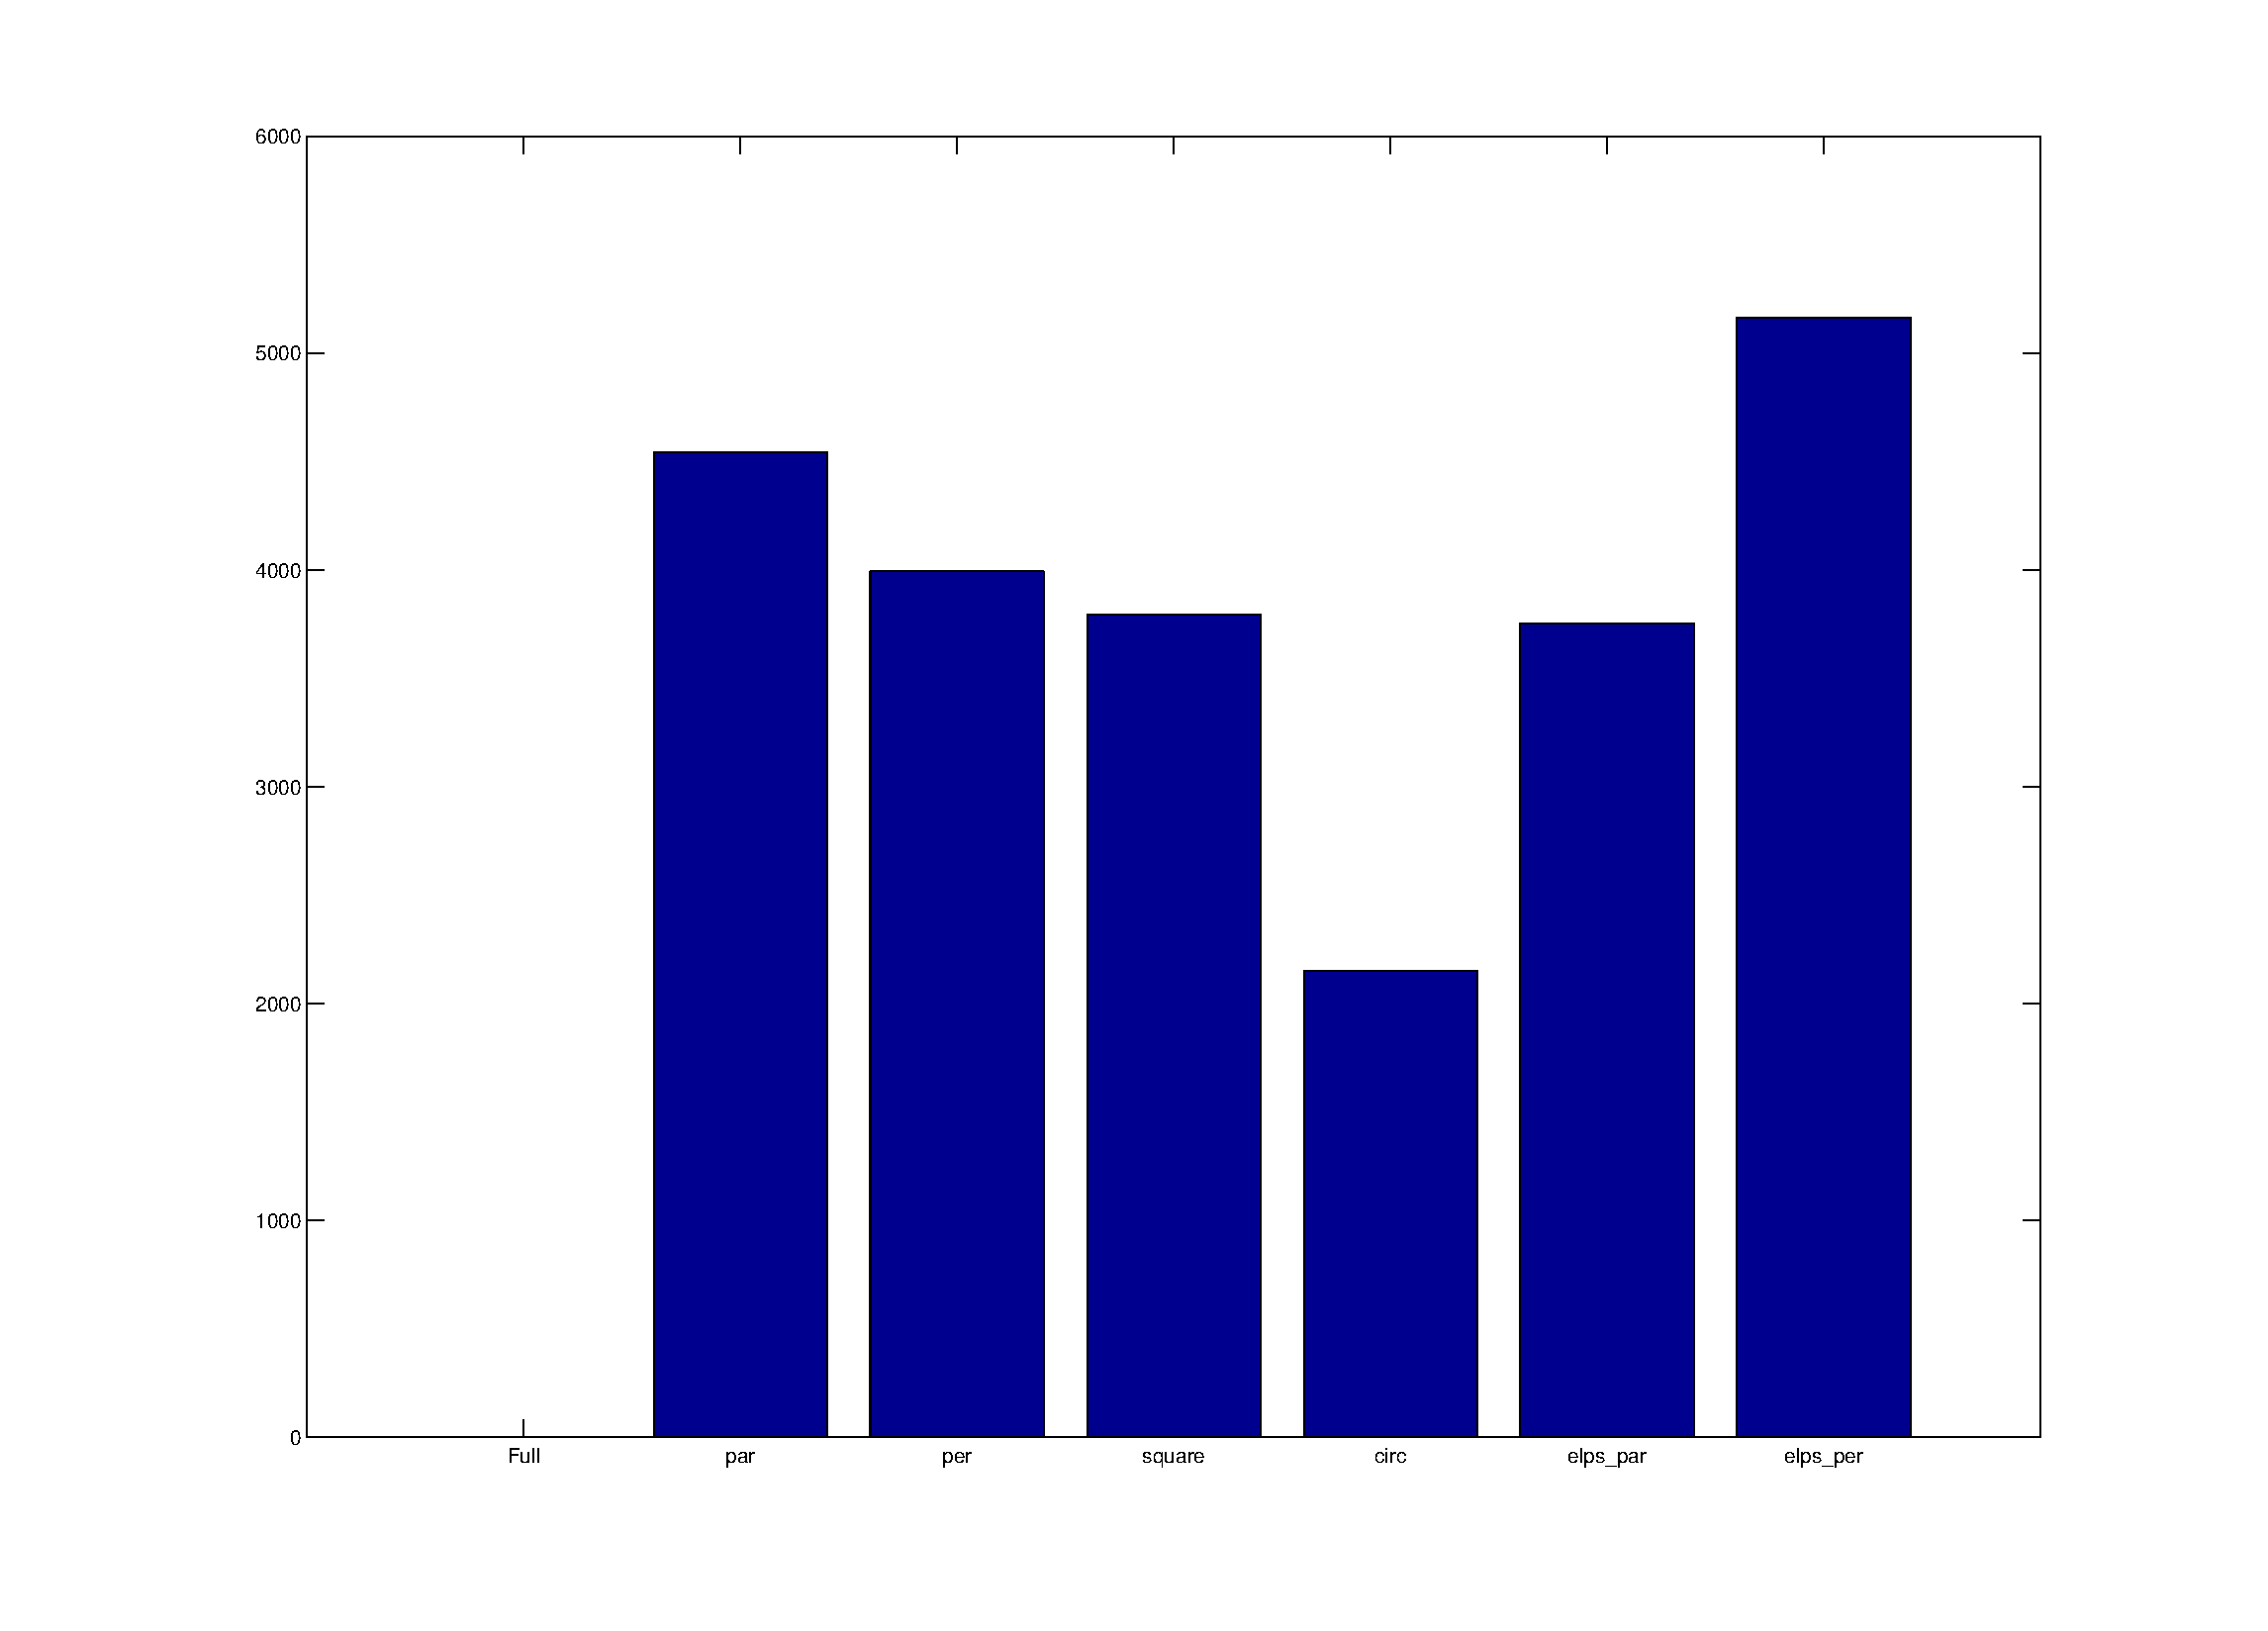
\includegraphics[trim = {10mm 0mm 10mm 0mm},clip,scale = 0.4] {Figs/numericalSims/brainRMS.eps}
        \caption{RMS error from fully sampled data in comparison to the fully sampled case.}
        \label{fig:RMSBrain}

        \end{figure}
    
  
  \subsection{Discussion}
  
    \noindent 03.25.15 - 04.01.15
    Surprisingly, we didn't particularly get what we expected. When running the simulation for the numerical phantom, the data didn't seem very different at all -- at least when comparing FA values. The data actually gave us results that were confounding... When being compared to the ``standard" methods of undersampling (i.e. Circular or low resolution undersampling), the parallel and perpendicular cases fell through and were not effective. However, even when looking for a ``happy medium" -- an elliptical technique, which we expect would have the lower RMS error of the circular technique, but the specificity of the directionally specific techniques -- we don't find that (with $n = 4$ for brains tested).
  
  
  \subsection{Other Notes}
  
    Due to space constraints, I've had to delete a lot of the (extraneous) data from the folders. I removed all of Jacob's recons (as they're unimportant, and stored elsewhere). I also deleted (inadvertently) the FA map that I produced for it, but all in all, it wasn't that important anyway. Since it is so easy to reproduce from the original information (i.e. the fully sampled case) I'm also getting rid of the undersampled real and imaginary data. 
  
  \subsection{Post-Meeting Notes}
  
    \emph{Meeting Date: 04.01.15}\\
    Brian stated that I should do some work on looking at the line profiles of everything that has been done because RMS is akin to looking primarily at DC information. This should give us a better rendition of what we want because we're interested in the edges more than the DC information. 



% Section IV
\section{Directional Continuum Sampling (04.14.15)}
  
  \noindent 04.14.15 -- Never completed
  \subsection{Preamble}
    
    \subsubsection{Basis}

      The idea behind what this method of acquisition is that we won't necessarily need CS for a reconstruction. The notion is to use a continuum of directions, as opposed to a specific number of discrete directions --  while only taking a small number of points for each ``direction" we would be able to do a full reconstruction using a solid angle of points (and possibly, be able to shrink the required number of points by utilizing CS). 
    
    \subsubsection{Meeting Notes}
      The notes are about building the simulation, as well as some work in relation to how to build the simulation. As of 04.14.15, I don't have a firm grasp of what I want to do and/or how I plan to do it. However, I believe that looking at PE tables (and including that in my solutions) will be a good method.
      \begin{itemize}
    	  \item If CS is to be used, incorporate the directional information before we look at 3D recon. A possible form could be:\\
    		\[ \me^{-\frac{\alpha_{jk}^2}{2\sigma^2}}\]
    		Where $\alpha_{jk} = \angle\vec{d_j}\vec{d_k}$
    	  \item Do a weighted average to obtain the proper eigenvalues for the simulation \\
        \end{itemize}
    
    \subsubsection{Meeting with Leigh}
      After meeting with Leigh SN to discuss methods of how to best do something that would make sense with respect to the FSE acquisition method. She pointed me to an email from Brian and the locations of some tables. 
      
      \bo{Email from Brian}\\
      	\texttt{Hello Jacob et al,}\\\\
      	  \texttt{You can try the following command for generation of cylindrical FSE tables.}\\\\
      	   \path{/home/bjnieman/source/vnmr/cyltable_gen.py --nf 64 --cylindrical --etl 8 --etlorder 2,1,0,3,4,5,6,7 --angorder 256 256 test_nf64_etl8_256_256}
           
           \hfill\\\\
      	    \texttt{Obviously, you can replace ``nf 64", ``etl 8", ``etlorder 2,1,0,3,4,5,6,7" and ``256 256" (as well as the output filename) with numbers of your choice. nf should be divisible by etl.}\\\\
            \texttt{To view the tables and inspect for problems, you can use:}\\\\
      	    \path{/home/bjnieman/source/vnmr/petable_display.py test_nf64_etl8_256_256_nf64_ni64}
            
            \hfill\\\\
      	    \texttt{Options -nacq and -etl <number> allow you to display the number of acquisitions (repeated in the table) or the echo number of each acquisition.}\\\\
      	    \texttt{Come to me if you have questions.}\\\\
      	\texttt{Brian}\\\\

      
      \bo{Email from Leigh}\\
      	\texttt{Here is the location of several different petables at 75 um (272 x 272 in the phase encode, $xz$ plane):}\\\\
          	\path{/home/leigh/cyltables/75um/angorder/LSN_E3_angorder_272_etl8_nf64_ni80}

      	    \path{/home/leigh/cyltables/75um/cylaxisdist/LSN_E3_cylaxisdist_272_etl8_nf64_ni80}

      	    \path{/home/leigh/cyltables/75um/pseudocyl/LSN_E3_pseudocyl_etl8_272_nf64_ni80}
            
      	    \texttt{If you need to look at all of the smaller tables (12 each) have a look in the parent folder, but know that there are a LOT of other tables in those folders, so just be careful to read the names carefully (they are different in the E3 E4 parts, where E3 means the third echo in the centre and E4 means the fourth).}\\\\
      	    \texttt{To make these tables I used the following commands:}\\\\
      	    \path{/home/bjnieman/source/vnmr/cyltable_gen.py --nf 64 --etl 8 --cylindrical --angorder --individ_table_limit 5120 --etlorder 2,1,0,3,4,5,6,7,8 272 272 --clobber LSN_E3_angorder_272_etl8}

      	    \path{/home/bjnieman/source/vnmr/cyltable_gen.py --nf 64 --etl 8 --cylindrical --cylaxisdist --individ_table_limit 5120 --etlorder 2,1,0,3,4,5,6,7,8 272 272 --cylaxisangle 90 --clobber LSN_E3_cylaxisdist_272_etl8}\\
            \texttt{NOTE, PSEUDOCYL IS A LITTLE DIFFERENT}\\\\
      	    \path{/home/bjnieman/source/vnmr/cyltable_gen.py --nf 64 --etl 8 --cylindrical --pseudocyl_pe2 --individ_table_limit 5120 --k0echo 3 --clobber 272 272 LSN_E3_pseudocyl_etl8_272}\\\\
      	    \texttt{Also, note that nf and the table axis (272) must be divisible by etl. These tables all have a resolution of 75 um.}\\\\
      	    \texttt{Let me know if you need anything else.}\\\\
      	\texttt{Leigh}\\\\

      These locations as listed above will be used in order to find the information about the PE tables so I make sure that what I do is compatible with the scanner -- thus I'm not testing something that can't be done. 



% Section V
\section{Return to CS with sparseMRI\_v0.2 (05.01.15 - 06.03.15)}

  \subsection{What happened?}

    When I was working with the code, at some point in time, I did something that fatally affected the code, causing problems and iterative work that would lead to results that were terrible -- equivalent to doing nothing at all. The CS reconstruction looked just like the zero-filled reconstruction. To figure this out, I re downloaded the codes and reran them, as I was having problems with the phantom reconstruction as well (which should work absolutely perfectly!). The code was re downloaded and placed in \verb!/micehome/asalerno/Documents/Lustig!.

  \subsection{Reanalysis and Understanding!}

    Here, I will discuss each code and exactly what's happening. The basis of the code will be from the \verb!demo_SheppLoganTV.m!, just like the previous time that I did this (which I will be looking at as a reference as well!), though this time, I will \emph{not} edit the code as much so that I don't break it again!

    \subsubsection{High Level Code}

      Note that the folder \verb!Orthogonal! needed to be added from Lustig's other code -- specifically the code that goes through Wavelets and their uses etc. \\

      \bo{p2DFT}:\\

        I don't quite get what the point of this is, though it seems like it's some sort of 2D Discrete Fourier Transform, in matrix form. This plays off of Brian's idea of using a matrix of matrices on the diagonal to apply this type of transform to the data.\\

      \bo{XFM}:\\
        This is the all important sparsifying transform. As a default it is set to be 1 for the phantom. For testing purposes, I will change this to be a wavelet. When this is run, using a Daubechies wavelet, at 6$^{\text{th}}$ order. As defined by Lustig, this means:

        \begin{quote}
       \texttt{The Daubechies filters are minimal phase filters that generate wavelets which have a minimal support for a given number of vanishing moments. They are indexed by their length, Par, which may be one of 4, 6, 8, 10, 12, 14, 16, 18 or 20. The number of vanishing moments is par/2.}
       \end{quote}

        \noindent Using the Wavelet transform, from a standard Shepp-Logan phantom, we get decent results! \\

      \bo{Eight Iteration \texttt{for} loop}\\

        Weirdly enough, this looks better as the iterations go on... It isn't running the \emph{exact} same thing each time, but using the previous data (seemingly) for each iteration. So, in theory, having a max of 64 iterations would be the same as having 8 iterations in the \texttt{for} loop with each loop having a max iteration limit of 8. This will be tested at some point -- go to it here. \\

      % \bo{Viewing}\\

       % After this, the rest of the code is just different ways to look at the images that come out of the code.\\
      \newpage
      \bo{Questions}

        \begin{enumerate}
          \item What exactly does the p2DFT do? Why use this instead of an FFT?
          \item What effects would different XFMs have (even using the same type, but with different numbers)?
          \item How do the two parameters that we have (soon to be made 3) affect the image?
          \end{enumerate}


    \subsubsection{Lower Level -- \texttt{fnlCg.m}}

      The prime importance of this part of the code is to understand \texttt{fnlCG.m} and the objective functions, because this is the basis of how everything is done in this code. By understanding this, I'll be able to build on it (or possibly even port it!).

      Originally, this code had all of the codes in one script, however, I moved all extra functions into their own scripts, located in the folder \texttt{./grads}.

      For this analysis, I will be switching between mathmode and verbatim. To make it easier, here are the switches:

      \begin{table}[h]
            \centering
            \begin{tabular}{| c || r | r | }
             \hline
             \textbf{Represents}                     & \textbf{Code}          & \textbf{Math Mode}          \\  \hline \hline
             \textbf{Raw Data} ($k$-space)           & \texttt{params.data}   & $y$                         \\  \hline
             \textbf{Image} (image-space)            & \texttt{XFM'*x}        & $m$                         \\  \hline
             \textbf{Iterative Data (sparse)}        & \texttt{x}             & $\Psi x$ or $\Psi m$                  \\  \hline
             \textbf{Fourier Transform}              & \texttt{params.FT}     & $\mathcal{F}_u[\cdot]$      \\  \hline
             \textbf{Sparsifying Transform}          & \texttt{params.XFM}    & $\Psi[\cdot]$               \\  \hline
             \textbf{Inverse Fourier Transform}      & \texttt{params.FT'}    & $\mathcal{F}_u^{-1}[\cdot]$ \\  \hline
             \textbf{Inverse Sparsifying Transform}  & \texttt{params.XFM'}   & $\Psi^{-1}[\cdot]$          \\  \hline
             \textbf{Gradient of the data}           & \texttt{dx}            & $\nabla \Psi m$          \\  \hline
            \end{tabular}
            \caption{Table of conversions between math mode and code.}
            \label{tab:conv}
            \end{table}

      \paragraph{What's Happening -- Superficially}

        The first thing that is done is looking at the line search parameters. These are parameters chosen for the minimization technique that's employed here. Nothing of major importance here since it is all set previously in the \texttt{params} variable.\\

        \subparagraph{Compute the gradient of the sparse data}

         The equation that we're editing is: $g_0 = \nabla\Psi(x)$
         This calculates the gradient of the \emph{sparse} dataset. It uses \texttt{wGradient.m}, which relies on calculation of the objective functions (which still needs to be discussed). \\\\

          \bo{\texttt{gOBJ.m} - Gradient of the Objective Function}
            
            \hfill\\
            \noindent This code is just one line:

            \verb!gradObj = 2*(params.XFM*(params.FT'*(params.FT*(params.XFM'*x) - params.data)));!. \\

            It is important to note that when the transform matrices are multiplied, it applies the transform, but multiplying by the transpose applies the inverse transform.

            The important players here are:
            \begin{itemize}
              \item \texttt{XFM} - The sparsifying transform
              \item \texttt{FT} - The Fourier Transform
              \item \texttt{x} - Our data that is undergoing iterations
              \item \texttt{data} - The original set of data
              \end{itemize}

            This line does the following:

            \begin{enumerate}
              \item Returns the data to image space
              \item Puts the data in $k$-space
              \item Subtracts the original dataset from it in $k$-space
              \item Returns the data to image space
              \item Puts image into sparse space
              \item Multiplies it by 2
              \end{enumerate}

            There's some intrinsic penalty right off the bat because of how the calculations are done. Firstly, with sharp edges, the FT's are not the exact same. In addition, the sparsifying transform likely has an effect.

            When looking at the phantom data, it seems that the major differences between \texttt{x} and \texttt{params.data} (not surprisingly) come from the edges, but the differences are decently sized ($\sim$0.5, compared to an image max of $\sim$1.)

            This code seems to do this part of the Compressed Sensing equations:

            \[ \left|\left| \mathcal{F}_u m - y \right|\right|_2 < \epsilon\]

            Since we are taking the \texttt{abs} of this when plotting (and looking at it's value in comparison to $\epsilon$) this is effectively taking the $\ell_2$ norm of the data.\\\\

          \bo{\texttt{gXFM.m} - Gradient of the $\ell_1$ Transform Operator}
            \hfill\\\\
            \noindent This function is also a one liner:\\

            \verb!grad = p*x.*(x.*conj(x)+params.l1Smooth).^(p/2-1);!\\

            \noindent Here, \texttt{p} represents the pNorm value for the $\ell_1$ term. It is a \emph{scalar} value!

            \noindent In mathematical notation (to be simpler to read) we have:

            \[ \nabla f = p x (|x|^2 + \alpha_1)^{\frac{p}{2} - 1}\]

            In this case, again, $x$ represents the sparsified data (i.e. it is in a sparse space) that continuously undergoes iterations. It's noted that $|x|^2 = x x^*$. $\alpha_1$ here represents an $\ell_1$ smoothing term. In the example here, it is set to be $10^{-15}$, and $p$ is set to be 1. 

            This equation doesn't seem to come up in the paper. If we analytically look at what this gives us, we can easily see what effect we should get. We will use the parameters as stated in the previous paragraph.
            \begin{align*}
              \nabla f &= p x (|x|^2 + \alpha_1)^{\frac{p}{2} - 1} & |x|^2 + \alpha_1 \approx |x|^2\\
                       &= x(|x|^2)^{\frac{1}{2} - 1}\\
                       &= x(|x|^2)^{-\frac{1}{2}}\\
                       &= x(|x|^{-1})\\
                       &= 1
              \end{align*}

            When we run the code, the difference between the range of values are $1 \pm 10^{-9}$. So we can see that the analysis makes sense. I will note, though, that I \emph{don't} get what this part does exactly. Brian and I \emph{NEED} to talk about this!\\

          \bo{\texttt{gTV.m} - Gradient of the TV operator}
            \hfill\\\\
            \noindent As the title says, this handles the TV operator. This, however, is more than one line, as the TV is applied to the data in \emph{image space}, but $x$ is iterated in the \emph{sparse space}.

            Something of interest is that when the TV operator is applied, the size of the matrix doubles, and increases a dimension! $x$ went from being [256 x 256] to [256 x 256 x 2]. There seems to be some orthogonality to it, as seen in \autoref{fig:TVOp}.

            \begin{figure}[!ht] 

              \centering
              \vspace{0pt}
              \setlength\fboxsep{0pt}
              \setlength\fboxrule{0.5pt}
              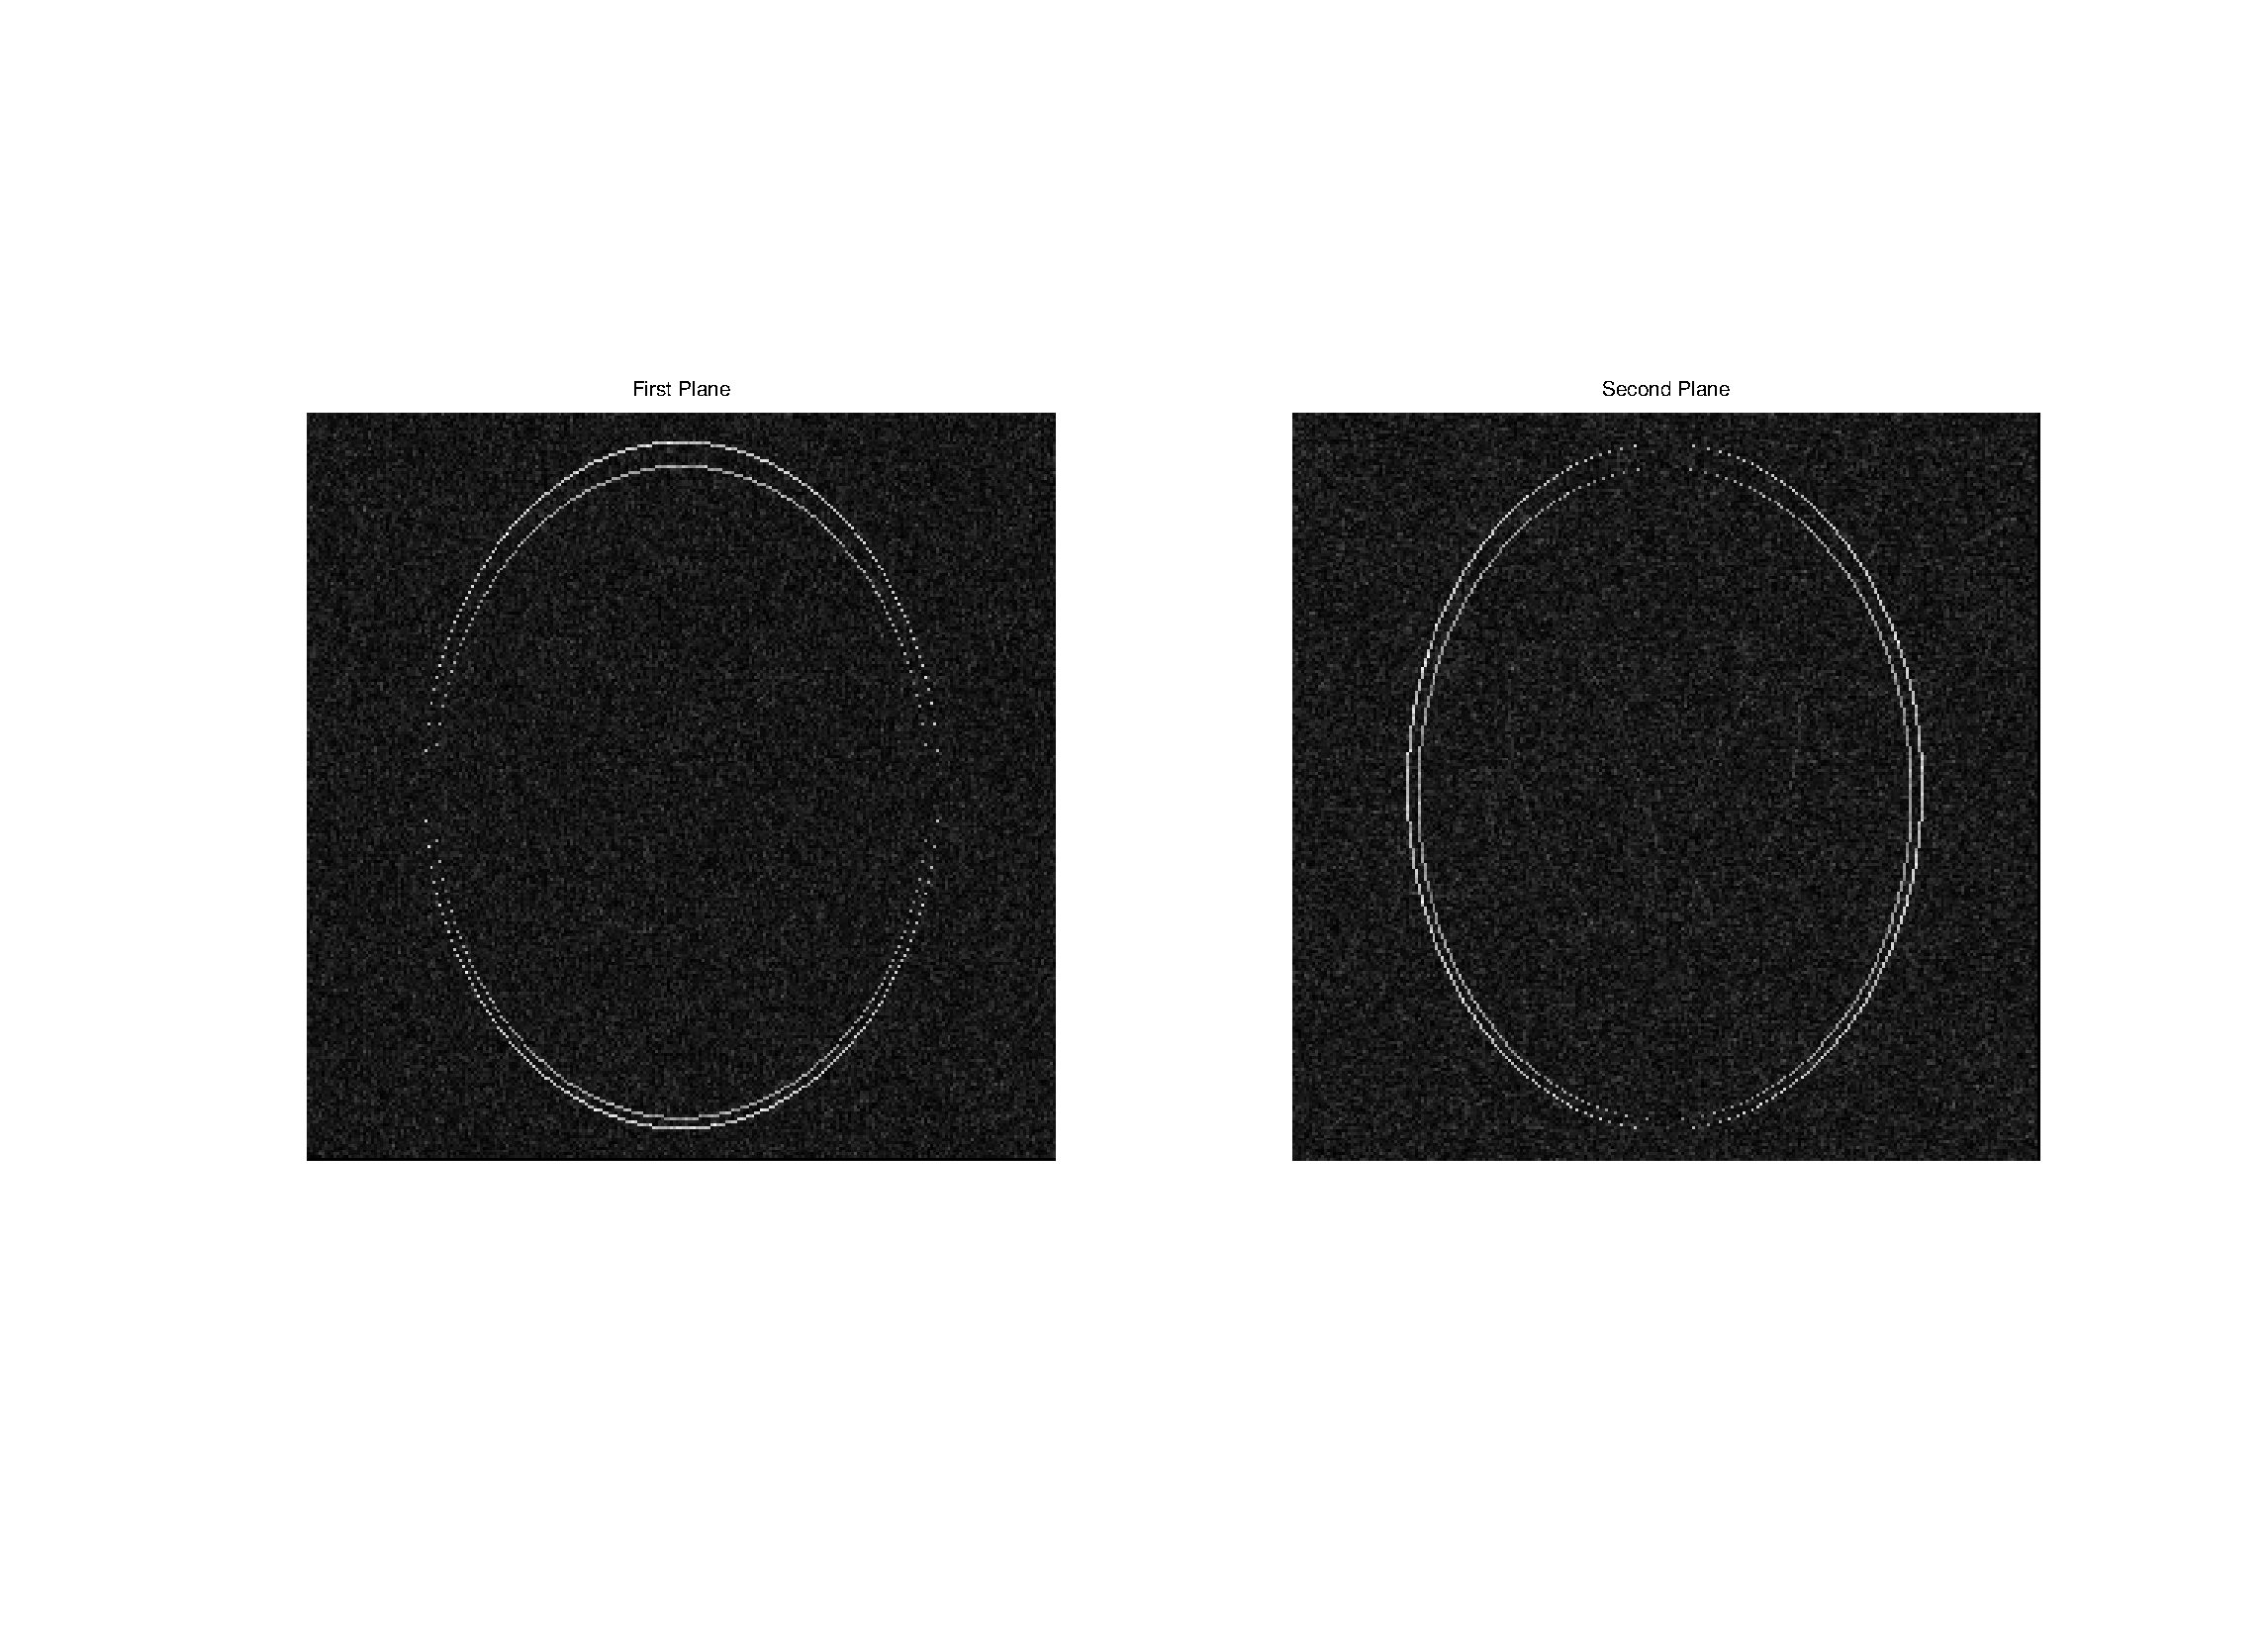
\includegraphics[trim = {20mm 60mm 20mm 50mm},clip,scale = 0.4] {Figs/CS_Code/TVOperated.eps}
              \caption{Comparison of the two [256 x 256] planes given in after the TV operator is applied}
              \label{fig:TVOp}

              \end{figure}

            Overall, however, this equation has a similar form to the one before it, but requires a few transforms in order to be put back into the sparse space.

            \noindent Let $D_x = TV[\Psi^{-1}[x]]$: 
            \[ \nabla f = \Psi[TV^{-1}[p D_x (|D_x|^2 + \alpha_1)^{\frac{p}{2} - 1}]]\]

            The terms inside of $\Psi[TV^{-1}[\dotsm]]$ are analogous to the terms in the above section. Again, we utilized $|D_x|^2 = D_x D_x^*$. In this case, however, it is noted that the data doesn't follow the same ``1" value as the \texttt{gXFM} did, even though the terms inside the transforms are all 1. My guess is that the noise of this distribution (which will happen in normal DAQ) will cause this value to increase dramatically (which is logical because variation will occur due to noise from voxel to voxel -- if it didn't, the assumption of Gaussian or Rician noise would be incorrect).\\

        \subparagraph{Compute the preobjective and objective}
          The preobjective (and objective) functions are calculated early in order to ``make it cheap to compute many times for efficient line-search". Some of these values are calculated many times and often, so this would be a good place to attack when we are looking at optimization.
          
          
          \bo{\texttt{preobjective.m} - Precalculates Transforms to Make the Line Search Cheap}
            \hfill\\\\
            This code is quite simple, as it just applies the transforms to both $x$ and $\diff x$ and places them in variables. The good news is that it makes them readily accessible, but the bad news is that in large datasets, this can become quite memory consuming. 

            The nomenclature is long, annoying, tedious, but all in all, understandable. The key is to look for each set of transforms. From this code, the outputs that we get are:
            \begin{itemize}
              \item \texttt{FTXFMtx} - $k$-space of $x$ ($\mathcal{F}_u[\Psi^{-1}[x]]$) 
              \item \texttt{FTXFMtdx} - $k$-space of $\diff x$ ($\mathcal{F}_u[\Psi^{-1}[\diff x]]$)
              \item \texttt{DXFMtx} - TV of the image space of $x$ ($TV[\Psi^{-1}[x]]$) 
              \item \texttt{DXFMtdx} - TV of the image space of $\diff x$  ($TV\Psi^{-1}[\diff x]]$)
              \end{itemize}

          \bo{\texttt{objective.m} - Calculates the Objective Function}
            \hfill\\\\
            The first thing that caught me in this code is the parameter $t$. It's just set to 1 in this code, but this adds \emph{yet another parameter} for us to play with. 

            \noindent In this code, we calculate the objective as:\\
            \verb!  obj = FTXFMtx + t*FTXFMtdx - params.data;!\\

            \noindent In mathematical terms, we have:
            \[ Obj = \sum\limits_{i=1}^N \left(\mathcal{F}_u[\Psi^{-1}[x]]_i + t\mathcal{F}_u[\Psi^{-1}[\diff x]]_i - y_i\right)^2 \]

            Where $y$ is the original data that we started with (off the scanner). We let $i$ represent the $i^{\text{th}}$ voxel of the data, since the objective value that we obtain is to be a measure of our loss. To put it into perspective, we are figuring out what the $\ell_2^2$ in $k$-space between the data, plus it's gradient, from the original data off the scanner. For all conversions, remember to see \autoref{tab:conv}.

            This then happens again for the XFM and TV differences, but in a slightly different manner, which will be explained below. 

            For those two, the code is as follows:

            \verb!w = x(:) + t*dx(:);!\\ 
            \verb!XFM = (w.*conj(w)+params.l1Smooth).^(p/2);!

            The only difference that exists between the two is what the \texttt{w} is calculated from. In \texttt{TV} it uses \texttt{DXFMt(d)x}, and in \texttt{XFM} it uses \texttt{(d)x}. This makes sense because the total variation uses the TV of image space (which is what \texttt{DXFMtx} is), and the \texttt{XFM} is calculated via the sparsified data, contained in \texttt{x}.

            The code was written in such a way that the TV and XFM weights don't need to be constant. The overall value given from the objective function is calculated as:

            \verb!res = obj + (TV) + (XFM) ;!

            Where the \texttt{TV} and \texttt{XFM} were multiplied by their respective weights. The RMS value is also calculated here, but it isn't used in \texttt{fnlCg.m}.

            This objective function is calculated once with $t=0$, as a reference, and then again with $t$ as a parameter -- the reference is used to break a loop. With $t = 0$, we lose all effects of the gradient, and so this is the differences that we would have with just the transforms (i.e. the problems I was talking about earlier because of the sharp edges and cutoffs, etc.).\\\\

          \bo{The importance of $\alpha$ and $\beta$}
            \hfill\\\\
            \verb!f1 > f0 - alpha*t*abs(g0(:)'*dx(:))!\\
            \verb!t = t*beta!\\

            \noindent \texttt{f1} is the value from the objective function when $t \neq 0$
            \noindent \texttt{f0} is the value from the objective function when $t = 0$.

            $\alpha$ and $\beta$ are very important in this analysis, as they give different weights when attempting to get out of the line search. 

            $\alpha$ tells us how strongly we will weight the effects of the gradient to take off of the original dataset if we wish to get comparable objective functions between the original dataset and the iterated dataset.  

            $\beta$ tells us how much are we going to weight the gradient when doing our calculations for the objective function. As we weight it less and less, we \emph{should} be getting closer and closer to the case where $t=0$, giving us smaller values.

            Once we get through the while loop via $\alpha$ and $\beta$ we update our data ($x$) and our gradients ($g_0$) and go through the calculations again with new starting criteria unless the $\ell_2$ of the gradient is less than $\epsilon$, or we've reached our iteration limit.

% Section VI
\section{Editing Lustig's Code (05.01.15 - 06.03.15)}

  For all of this work, the code has been moved to \texttt{CompressedSensing} -- anything from the aforementioned \texttt{CompressedSensing} folder has been moved to \texttt{MincMatlab} for a better naming scheme.  A ``safe version" of the code can be found in \texttt{Lustig/sparseMRI\_v0.2}.

  For all of this code, the expectation is that from the data, we will have it separated by slice in the readout direction and then stacked by direction. So in a (preferably \texttt{.mat}) file, we would have one brain, one readout slice, all directions. Note that (for obvious reasons), the order of the directions should be the same as in the Gradient Vector file.

  Currently using \texttt{for} loops, which is relatively slow -- but will work to check brute force calculations for right now. I'll be doing this a la John Camarack, and optimizing later -- \texttt{mtimesx} may be a good place to look for optimization routines...
  
  \subsection{Meeting With Brian (05/06/15)}
    Brian has some ideas for what needs to be changed. It can be looked at as a few points.
    \begin{itemize}
      \item Weighting Function
      \item Phase Correction
        \begin{itemize}
          \item Undersampled recon and smooth it out and look at the phase 
          $
          \theta = \tan^{-1}
          \left(
          \frac{\text{Im}(x_{ij})}
               {\text{Re}(x_{ij})}
               \right)
          $
          \item Generally, the phase correction that Leigh will apply should be done before this (this one makes sure that the phase is generally okay before we do anything else)
          \end{itemize}

      \item Make this work for multiple directions -- i.e. adapt the code to work in 3D
      \end{itemize}


  \subsection{Phase Correction}
    As per Brian, the way to calculate the phase would be to take the image (as it is real and imaginary) and do:

    \[ P = \frac{s^*}{|s|} \]

    Where $s$ represents the signal of the image. This is akin to multiplying by $\me^{-\Psi(s)}$.

    When I run the calculation using the above equation, it looks \emph{nothing} like what Lustig gets through his method. So, I want to talk this through with Brian, and see exactly what the best method here -- is what I'm doing correct?! Calculations for the phase can either be done Brian's or Lustig's way -- and can be found in \texttt{phCalc.m}. Currently, the code will do the phase calculation either way, based on \texttt{rl}, a parameter that is fed into it. 

    I ran a quick check, testing the phase for different slices, and determined that (with the exception of the areas of zero-padding) the phases are different. 

    Via a quick reality check, I made a file \texttt{brain.6.01.mat} that is zero-padded, but only the first direction (as opposed to all directions in \texttt{brain6.mat}).

  \subsection{Weighting Function}
    We want the code to be able to work on all 30 directions simultaneously and have them be weighted according to how similar the gradient directions are. In order to make sure that this is absolutely viable, some minor edits had to be made to the \texttt{GradientVector.txt} file in order to make the magnitude of each vector as close to 1 as we can get them (currently, they are correct to $1 \pm 0.004$). 

    The weighting function that we are planning on using has the form:
    \[ \alpha = 
    \me^
    {-\frac{(\vec{d_i}\cdot\vec{d_j})^2 - 1}{2\sigma^2}} \]

    A code for this is written, it is called \texttt{dotThresh.m}. It can be found in \texttt{./diffusion}. 


  \subsection{Diffusion Direction based ``Gradient" -- Directional Redundancy}
    Here is where we look at the actual directional redundancy that we get when using the many different (and similar) directions. 

    All of the gradient codes were edited to work with all 30 (or however amount) of directions that we have. Again, the expectation is that the brains are split into a different file for each slice about the readout, and each stacked image is a different direction. 

  \subsection{Problems}
    Noticed that when running the objective function, my error is astronomical ($\sim 10^{13}$), so I decided to do a check with Lustig's and his is MUCH lower. So I'm doing some reality checking with the first direction. Essentially, I ran the Lustig's \emph{vanilla} code with this slice, and am comparing it to the results of my altered version.

    When running the two, the FT's are identical, as are the XFM's (as they are well defined). The error, I believe, must come from the TV... 

    Nope. In fact, the major difference is occurring with the directional weighting (duh!) because it is actually comparable in size to gradObj, ($\sim 10^2 - 10^3$), while the other two are much smaller ($\sim 10^{-2} - 10^{-1}$).

    Turns out I made a stupid mistake and was dividing by the PDF in the \texttt{res} calculation! Edited this, and now all is well! Need to be more careful.

    What I've noticed is that the directional differences are significantly more varied than the others. We have differences varying from $10^{-33}$ to $10^{22}$. Could this be due to very different images, or possibly due to relatively different dot products (i.e. $\vec{d_i}\cdot\vec{d_j} \approx 0.25$), but the weighting isn't dropping fast enough. 

    The code is SLOW. When I run a 2D test in comparison to the original, it takes about 2 seconds longer. The 3D version takes very long. I'm testing it in comparison to looping the 2D case. 

%section VII
\section{Continuation of Editing -- Post-Vacation (06.10.15 - 07.17.15)}
  
  Took a vacation and have been slacking with regards to entering my notes in here. As a quick update as to what's going on, I have the following:

  The code is up and running -- right now we are doing some parameter optimization with respect to $\lambda_{1,2,3}$. This took much longer than anticipated because of some errors that I made with respect to the data. The data wasn't FFT'd properly, causing there to be a ``chequerboard"pattern on it -- that is, all high frequency information. This was causing the sparsity constraint to fail miserably, as all of the information after the wavelet was in the bottom right corner, instead of the top left (this is because the wavelets are actually only working on the real part of the data). 

  As of now, everything is looking a bit better, however, there still does seem to be this soft roll in the data... Could this possibly be due to a misplacing of ``zero" in the transition from \texttt{vrecon} to \textsc{Matlab}?

  \subsection{Comparison to Fully Sampled}
    For this section, the comparison that was done was between the data that comes out of the algorithm, and the original fully sampled data. It is noted that both sets of data have individual voxel values on the order of $10^4$. The overall RMS difference that we get between the datasets (for a $256 \times 256$ dataset) is also on the order of $10^3 - 10^4$.

    What I've found (which as of right now needs to be confirmed), is that there are sections that are slightly better than others -- though not by much. These sections come up in sort of ``waves" within the parameter optimization map. Below is an optimization map, done using a logarithmic map for \texttt{xfmWeights} and \texttt{TVWeights}. We can see that is seems like there are jump discontinuities, but these are not as big as they seem in \autoref{fig:lamOpt}. The dynamic range of the colour axis only spans a value of less than 200, for an RMS average of about $8 \times 10^3$, or about $10^{-1}$ for each voxel! In \autoref{fig:lamOptHigh}, we can see a similar plot, but the XFM and TV values are much higher.This leads to a slight increase in the RMS, but the XFM and TV differences in the objective function are comparable to the OBJ (the $\ell_2$ norm) of the data consistency term. This is what we're looking to get, as it's what is seen in the Shepp-Logan example.

    \begin{figure}[!ht] 
      \centering
      \vspace{0pt}
      \setlength\fboxsep{0pt}
      \setlength\fboxrule{0.5pt}
      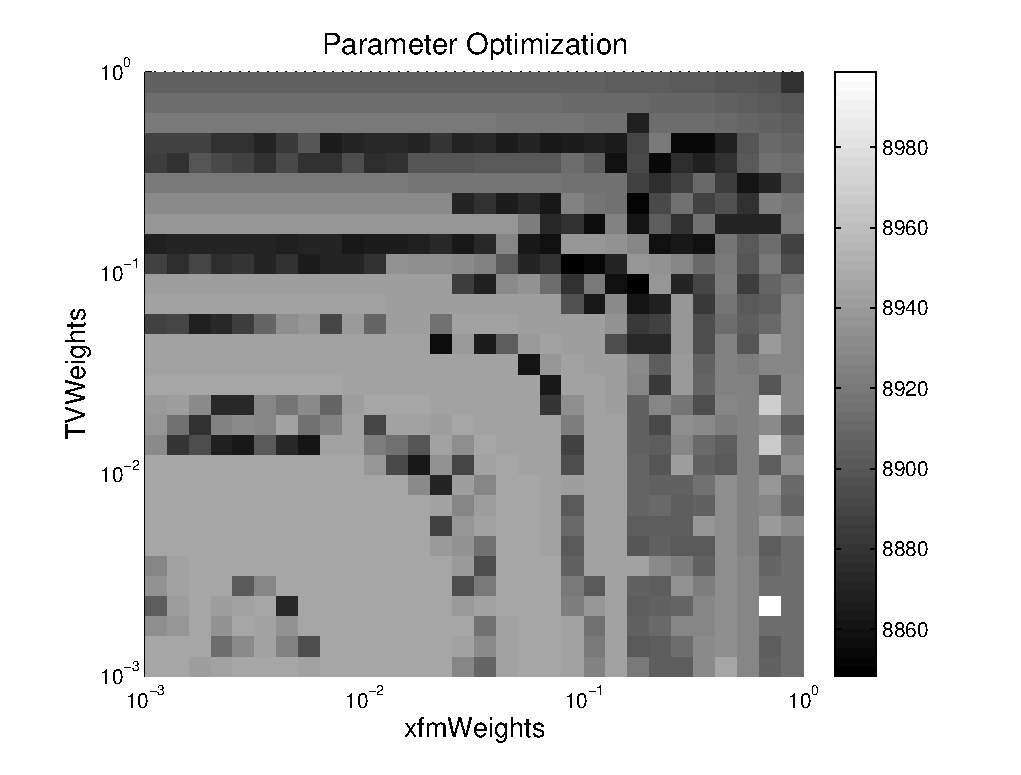
\includegraphics[trim = {0mm 0mm 0mm 0mm},clip,scale = 0.4] {Figs/CS_Code/ParamOptimization.eps}
      \caption{Parameter optimization using an RMS difference. These values are computed using TV and XFM $\in [10^{-3},1]$. Classified as the ``low" parameter values. }
      \label{fig:lamOpt}
      \end{figure}

    \begin{figure}[!ht] 
      \centering
      \vspace{0pt}
      \setlength\fboxsep{0pt}
      \setlength\fboxrule{0.5pt}
      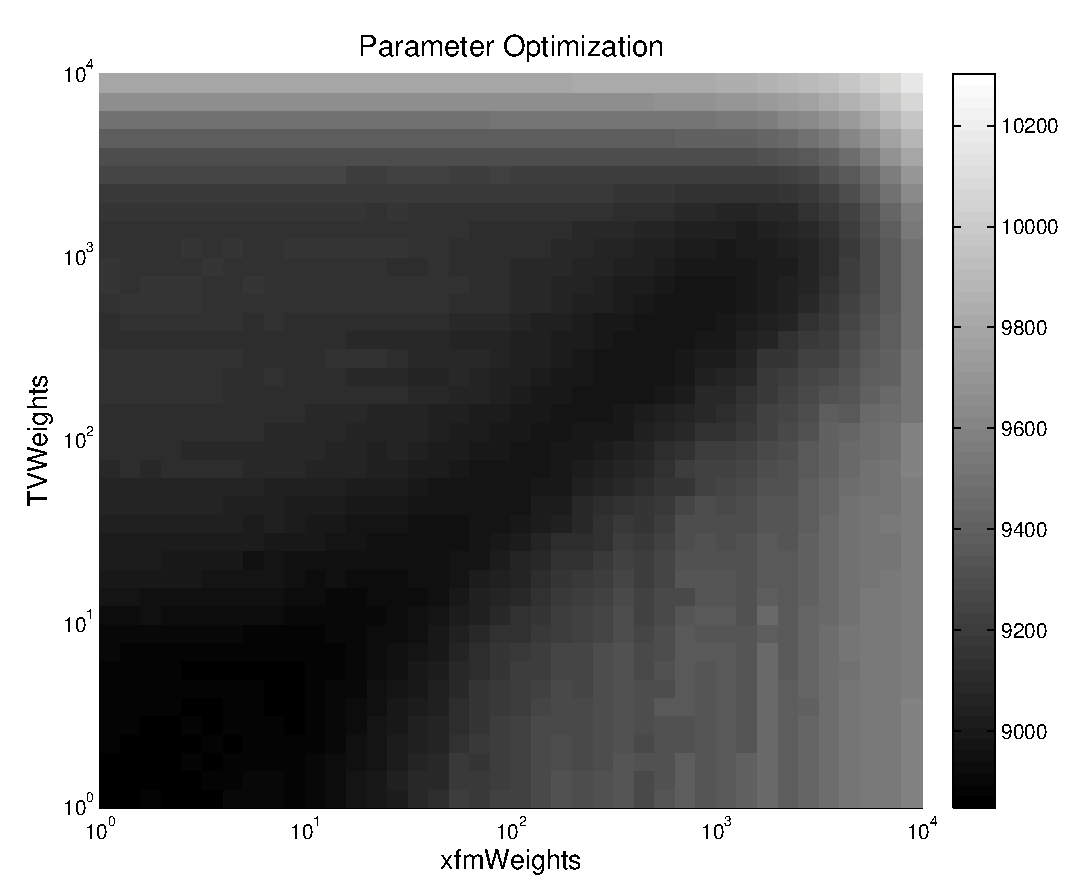
\includegraphics[trim = {0mm 0mm 0mm 0mm},clip,scale = 0.4] {Figs/CS_Code/ParamOptimization-HighTVxfm.eps}
      \caption{Parameter optimization using an RMS difference. These values are computed using TV and XFM $\in [1,10^{4}]$. Classified as the ``high" parameter values.}
      \label{fig:lamOptHigh}
      \end{figure}

  \subsection{What next?}
    After looking at all of the figures, what I've found is that they don't seem to be very different from each other if we look at the magnitude of the images. It is noted that they do look pretty nice, and in my eyes better than the merely undersampled case. I want to analyse a few things after looking at these images:
    
    \begin{itemize}
      \item Can we even more grossly undersample in order to see weirder effects?
      
      \item How different are the images actually? Is one of the parameters better to change for differences? Were the values that I chose to work with too close together (i.e. it was taking $\lambda_{1,2} \approx 0$)?

      \item What exactly is the distribution of the noise? We've added in incoherence noise, and removed some noise via denoising steps in the algorithm.

      \end{itemize}
    \subsubsection{Parameter Weighting}
      Something that I noticed when running the same analysis on the Shepp-Logan phantom was that the XFM and TV weightings are actually close to the objective weighting, $\pm$ an order of magnitude. This is integral information to have, because of how it compares to the case of our data, where it is many orders of magnitude lower. Perhaps we are not using the right orders of values for our analysis -- this may be why we see such minuscule differences when we change our parameters.

      The data for each section can be found easily. The low parameter data can be found at \path{/projects/muisjes/asalerno/CS/data/LowTV-XFM.mat}, and the high data can be found at \path{/projects/muisjes/asalerno/CS/data/HighTV-XFM.mat}. Each of these is a 4D file, where the 3$^{\text{rd}}$ dimension is TV and the 4$^{\text{th}}$ dimension is XFM weights. In each dataset, the xfmWeights and TVWeights variables can be found. This is useful if you are using something like \texttt{logim.m} to plot. \\

  \subsubsection{Meeting Notes -- 06/24/15}
    During my meeting, Brian suggested that I change how the images are input into the algorithm. The benefit of this is that ``no matter what we feed into the code, the parameters should still be the same". 

    Brian also wants me to normalize the data so that either the images' maxima are set to be 1, or that  $(k_x,k_y) = (0,0)$ has a value of 1. This also means that $\bar{\text{im}} = 1$. 

    Eventually, Brian wants to fix this value so that we don't have this drop in intensity when applying CS to diffusion data. An idea is to either: 

    \begin{itemize}
      \item Add in another term of the form $(F_o - \int{f(x)\diff x)^2}$ where $f(x)$ is the image, and $F_o$ is the original average.
      \item Possibly tack on a weighting term: $||w (\mathcal{F}_u\{f(x)\} - y)||_2$
      \end{itemize}

    Later on, an idea may be to work in $k$-space! Problem with this, however, is that we would have to properly apply $\mathcal{F}{\nabla f(x)}$. Again, here, $f(x)$ is the image. 

    Lastly, with respect to the noise analysis (talked about later, in Section 7.3) I was able to show that the noise looked Rayleigh (and thus likely Rician). However, Brian said to look into this more by analyzing the $\mathds{R}$ and $\mathds{I}$ parts individually to check if they're both Gaussian. 

  
  \subsubsection{Normalization -- 06/29/15 - 06/30/15}

    I did a quick test of this, and it seems like by doing this, we can get the more realistic (and noted in literature) values of $\lambda_{1,2} \leq 1$. However, we still hit a pretty big issue, \emph{the DC component seems to push for the very low values of $\lambda_{1,2}$, even though visually, they're not necessarily the best.} For this, Brian suggested to look at the zero-point of $k$-space. This may be a good idea regardless, as it seems like there may be a light roll off where there shouldn't be in the raw image data -- it can be seen in the real part of the data. 

    As of 06/29/15, this has been fixed, however the original data has been put in \path{/projects/muisjes/asalerno/CS/data/raw_test_data/data}. The issue that existed was that for a 256 $\times$ 256 dataset, the $(k_x,k_y) = (0,0)$ was not in the proper location. 

    It seems like the data is now well normalized and there actually isn't a drop in the mean of the data after applying the CS routine. The \emph{max} seems to drop, but the mean actually increases by a fraction of a percent. The code \path{/home/asalerno/Documents/CompressedSensing/demo_TVxfm.m} has been edited in order to include the ability to normalize either by max or mean. \\

    \bo{06/30/15}\\\\

    Something interesting that I noted was that the first iteration performs the most ``clean up" of the data. If one were to run the code, looking at the data after each loop, I'd expect that they'd see a major jump after the first run, then the differences to taper off exponentially after that -- like a power function. 


  \subsection{Noise Analysis}
    By taking a small subset of the image where the noise exists, I ran a simple noise analysis on the data. The noise analysis that was done is akin to the one done in MBP 1024 for the MRI lab. In fact, it uses a slightly modified version of that code. 

    When this analysis was done, it appears as if the noise is Rayleigh distributed \emph{after} the Compressed Sensing algorithm, regardless of the parameter choice (under $\lambda_{1,2} \in [10^{-3},1]$ -- the same analysis is to be done for $\lambda_{1,2} \in [1, 10^4]$. To test this, I ran the analysis on each image coming out of the parameter optimization algorithm. The noise distributions were fit to a Lorentzian, Gaussian, and Rayleigh function, with the highest value of an adjusted R$^2$ value taken to be the ``best fit".

    Doing the same analysis for the data before the compressed sensing algorithm, we find that, again, we exist in a low SNR regime of MRI where the data fits nicely to a Rayleigh function. Thus, I believe it is OK to utilize our normal statistics on the data. 

  \subsection{Overly Smoothed Results with $\lambda_1 = \lambda_2 = 0$ -- 06/30/15}

    \begin{figure}[!ht] 
      \centering
      \vspace{0pt}
      \setlength\fboxsep{0pt}
      \setlength\fboxrule{0.5pt}
      \includegraphics[trim = {0mm 0mm 0mm 0mm},clip,scale = 0.4] {Figs/CS_Code/overSmooth.eps}
      \caption{Overly smoothed result. Comparisons of when there is no compressed sensing, to when $\lambda_1 = \lambda_2 = 0$, and again to $\lambda_1,\lambda_2 \neq 0$}
      \label{fig:overSmooth}
      \end{figure}

    Some weird results are occurring when $\lambda_1 = \lambda_2 = 0$. Essentially, we'd expect that we end up with something that is very close to the original dataset, as can be seen in the figure above. However, this isn't the case -- we are obtaining an overly smoothed result that looks almost nothing like the original \texttt{im\_dc}
    variable as we would expect. The question here is why. 

    Looked into whether it was the XFM that was causing it. Upon some quick inspection, I can safely say it wasn't. On the first iteration, when it goes through the line $x = x + t*\diff x$, the major difference comes. Somewhere in this line is a major change that occurs. The question, however, is exactly what is happening... 

    Apparently, FTXFMtx looks quite a lot like a brain (as it should as it's apparently just the $k$-space image of the brain)... This could be where we're getting the utter craziness. Is this what is building our first guess? Perhaps our first guess is a very smoothed out version of the data that we have. 

    As of 06/30/15, we've figured out that the issue actually arises from what exactly is being taken as \texttt{im\_res} and \texttt{data}. Because of this, we have many different angles that we have to look at.


  \subsection{Analysis of the code -- What's our starting point? -- 07/02/15 - 07/17/15 }

    \bo{07/02/15}\\

    Looked at the code and found how similar the data looks right from the get go -- the basis that we are using is \texttt{data}, even though the data that we are feeding into it is \texttt{im\_dc}, which is density compensated. Thus, after the first iteration, it's being pushed towards the non-density-compensated case. Thus, even when $\lambda_1 = \lambda_2 = 0$, we get this nicely smoothed image. \\

    \bo{07/03/15}
    
    Looking into this a little more, I want to see exactly when the data tanks towards the \texttt{data} variable, i.e. when there is no density compensation. 
  

% Section VIII
\section{Adding in the Directional Component -- 07/17/15 - 08/20/15}
  
  \subsection{Directionally specific sampling -- 07/20/15}
    After going through the code and figuring some stuff out about $\lambda_1 \& \lambda_2$, we thought it would be a good idea to continue on and go with the directional component of the undersampling.

    \subsubsection{Directional Undersampling with a Cause}
      This part of the project was a bit more difficult than I had first thought it would be. The problem presented itself as the fact that we have 30 directions and we want to undersample in such a way that over some small solid angle we can have a fully sampled brain. 

      In order to do this, I had to start with the system of looking at the minimum energy in an electrostatics point of view. There are ways to do this with a continuum of directions (talk to Jan about the applet). However, for the fact that we have our 30 directions, we can't use this system. So I went through all $_{30}C_k$ combinations (where $k = \lfloor 30 p \rfloor$)
      
      Using this method of undersampling, I was able to get a good rendition of the original fully sampled dataspace. \emph{However, this MUST BE TAKEN WITH A GRAIN OF SALT}. The reason for this is that we are looking for minute differences in data, so, how much better does adding directions that are very similar do in comparison to adding in directions that are very different. I will do an analysis on this in another section.


% Section IX
\section{Committee Meeting Notes -- What is my future plan?}

  In my committee meeting, I was told a few things. Some good, some that I need to take a deeper look at. Primarily, the notion is that I will be able to finish within a reasonable amount of time -- and I plan to do so. 

  Given what I showed the group, specifically pertaining to a two-fold approach with respect to direction -- namely using it as an extra term in the equation as well as a specific method of undersampling -- there were some notes that were made:

  \begin{enumerate}
    \item Consider a sparsity transform in angular space -- an idea for this could be a ridgelet transform.

    \item Link total variation in space and angle -- this will make the ``extra term" that we tack on more mathematically believable

    \item Investigate using angular term \emph{alone} in recon -- this will help me figure out exactly what this term is doing in the reconstruction method

    \item Test higher compression factors -- how far can we push this before it breaks down?

    \item Verify convergence across multiple starting conditions -- Does the starting point matter in how this will work? If so, we need to take a step back and look at the code closely

    \item Improve metric for evaluating results -- this is very important, as right now, all we use is an RMS, which may not be super accurate.
    \end{enumerate}
  
  In addition to these notes, I \emph{really} need to be better at knowledge of neuroanatomy, clinical applications of DTI, other imaging/neuroscience research methods.


% Section X
\section{Post Committee Meeting Work}

  \subsection{Analysis of the Angular Term in the Reconstruction}
    Specifically, the term that I'm talking about here is the extra term that we tacked on. The equation is $w_{i,j} \sum\limits_{\substack{i,j = 1 \\ i \neq j}}^n  \me^{{-\frac{(\vec{d_i}\cdot\vec{d_j})^2 - 1}{2\sigma^2}}}$ Chris Macgowan suggested that I go through and see exactly what the extra term does \emph{on it's own}. It's noted that this will take a while because of how the recon is done.

    There are a few parameters that we have control over.


\end{document}